%%%% DOCUMENT CLASS ************************************************************
\documentclass[print,thumbmain,final]{src/thesis}  % uncomment for writing
%\documentclass[final]{src/thesis} % uncomment for rendering/final version

%%%% PREAMBLE ******************************************************************
%!TEX root = ../thesis.tex
%\usepackage{amsmath}
\usepackage[fleqn]{amsmath}
\usepackage{amsfonts}
\usepackage{amssymb}
\usepackage{accents}
\usepackage{amsthm}
\usepackage{appendix}
\usepackage{afterpage}
\usepackage{array}
\usepackage[dutch,english]{babel}
\usepackage[autostyle]{csquotes}
\usepackage{enumitem}
\usepackage{epsfig}
\usepackage{epstopdf}
\usepackage{fancyhdr}
\usepackage{float}
\usepackage{graphicx}
\usepackage{lipsum}
\usepackage{longtable}
\usepackage{multicol}
\usepackage{multirow}
\usepackage[numbers,sort&compress]{natbib}
\usepackage[final]{pdfpages}
\usepackage{relsize}
\usepackage{subfig}
\usepackage{siunitx}

\usepackage{tcolorbox}
\usepackage{thmtools}
\usepackage{todonotes}
%\usepackage{tikz}      % The tikz package is added in mrthesis.cls for producing thumbindex
\usepackage{url}
\usepackage{xcolor}
\usepackage{textcomp}

\usepackage[bookmarks=true,bookmarksopen=false,colorlinks=true,pdfpagelayout=TwoColumnRight]{hyperref}
\hypersetup{
    colorlinks,%
    citecolor=black,%
    colorlinks=true,%
    filecolor=black,%
    linkcolor=black,%
    urlcolor=gray,
    }
\usepackage{bookmark}

\setlength{\mathindent}{1.75cm}

%!TEX root = ../thesis.tex

% Texts or
\newcommand{\ie}{\textit{i.e.}}
\newcommand{\eg}{\textit{e.g.}}
\newcommand{\blank}{\,\cdot\,}
\renewcommand{\emph}[1]{'\textit{#1}'}
\newcommand{\sorotoki}{\textup{\texttt{SOROTOKI}} }
\newcommand{\matlab}{\textup{\texttt{MATLAB}} }
\newcommand{\data}[1]{(\raisebox{-2.7pt}{\textcolor{#1}{\,\Huge{\textbf{-}}}})}
\newcommand{\ldata}[1]{\raisebox{-2.7pt}{\textcolor{#1}{\,\Huge{\textbf{-}}}}}

% Equations/math
\newcommand{\be}{\begin{equation}}
\newcommand{\ee}{\end{equation}}
\newcommand{\benn}{\begin{equation*}}
\newcommand{\eenn}{\end{equation*}}
\newcommand{\bea}{\begin{eqnarray}}
\newcommand{\eea}{\end{eqnarray}}
\newcommand{\beann}{\begin{eqnarray*}}
\newcommand{\eeann}{\end{eqnarray*}}
\newcommand{\ba}{\begin{align}}
\newcommand{\ea}{\end{align}}
\newcommand{\bpm}{\begin{pmatrix}}
\newcommand{\epm}{\end{pmatrix}}
\newcommand{\bbm}{\begin{bmatrix}}
\newcommand{\ebm}{\end{bmatrix}}
\newcommand{\bc}{\begin{center}}
\newcommand{\ec}{\end{center}}
\newcommand{\pwr}[1]{\cdot10^{\textrm{#1}}}

% Symbols and annotations
%\newcommand{\fB}{\boldsymbol{f}}
\newcommand{\maT}{\text{ma}}
\newcommand{\qR}{\mathrm{q}}
\newcommand{\RBB}{\mathbb{R}}
\newcommand{\rmsT}{\text{rms}}
\newcommand{\xBF}{\mathbf{x}}
\newcommand{\interior}{\operatorname{int}}

% Tikz figures
\newcommand{\SF}{1}                 % Scaling factor
\newcommand{\TS}{\normalsize}       % Text size
\newcommand{\lw}{0.7pt}             % Line width
\newcommand{\TSTick}{\small}        % Text size axis labels
\newcommand{\axislabels}[2]{\foreach \x/\y/\s in {#1} {\node[#2,inner sep=1mm] at (\x,\y) {\TSTick $\s$};}}
\newcommand{\wheel}[3]{ \draw[line width=\lw] (#1,#2) circle (#3);
                        \fill[bottom color=MRblue!60!black!80,top color=MRblue!10] (#1,#2) circle (#3-0.5*\lw);
                        \fill[color=MRblue!30] (#1,#2) circle (#3-\lw);
                        \fill[top color=MRblue!60!black!80,bottom color=MRblue!10] (#1,#2) circle (0.7*#3);
                        \fill[color=MRblue!30] (#1,#2) circle (0.7*#3-\lw);
                        \fill[color=black] (#1,#2) circle (0.1*#3);}

\newcommand{\CoM}[3]{\filldraw[inner color=white,outer color=black!7!white,draw=black,line width=\lw] (#1,#2) circle (#3+0.5*\lw);
                     \begin{scope}[xshift=#1,yshift=#2]
                        \clip(-#3,0) -- (0,0) -- (0,#3) -- (#3,#3) -- (#3,0) -- (0,0) -- (0,-#3) -- (-#3,-#3) -- cycle;
                        \fill[inner color=black!50!white,outer color=black] (0,0) circle (#3);
                     \end{scope}}

\definecolor{MRdarkblue}{RGB}{16,9,88}      % Define a set of colors to be used throughout thesis
\definecolor{MRred}{RGB}{152,0,0}
\definecolor{MRgreen}{RGB}{0,146,69}
\definecolor{MRblue}{RGB}{53,153,204}
\definecolor{MRorange}{RGB}{220,85,30}
\definecolor{MRlightgreen}{RGB}{217,224,33}
\definecolor{MRyellow}{RGB}{255,214,0}
\definecolor{MRgrey}{gray}{0.95}
\usetikzlibrary{arrows}
\usetikzlibrary{patterns}
\usetikzlibrary{decorations.markings}
\usetikzlibrary{shadings}
\usetikzlibrary{shapes}

% Counters
\newcounter{ContNum}        % Counter for the contributions
\renewcommand{\theContNum}{\Roman{ContNum}}

% Other
\newcommand\blankfootnote[1]{%
  \let\thefootnote\relax\footnotetext{#1}%
  \let\thefootnote\svthefootnote%
}
\newcounter{numfootnote}
\newcommand\numfootnote[1]{%
    \stepcounter{numfootnote}%
    \newcommand{\thefootnote}{\thenumfootnote}%
    \footnote{#1}
}

\newcommand{\disclaimer}{\\[\baselineskip]  A detailed list of the differences between this chapter and the article on which it is based is provided in the %\hyperref[chap: Modifications]{\emph{Modifications}}
\emph{Modifications} chapter of this thesis.}
\newcommand{\itemheader}[1]{~\\ \noindent\textbf{#1.}\ \ }
\newcommand{\itemheaderNewpage}[1]{\newpage \noindent\textbf{#1.}\ \ }
\newcommand{\contribution}[2]{\refstepcounter{ContNum}#2 \vspace*{2.1mm}\begin{tcolorbox}[colback=black!2!white,colframe=black!20!white] \textbf{Contribution \Roman{ContNum}.} {\em #1} \end{tcolorbox}\vspace*{2.1mm}}
\newcommand{\objective}[1]{\begin{tcolorbox}[colback=black!2!white,colframe=black!20!white] {\em #1} \end{tcolorbox}}
\newcommand{\terminology}[2]{\begin{tcolorbox}[colback=black!2!white,colframe=black!20!white] {\textbf{Terminology: } \textbf{#1} \em #2} \end{tcolorbox}}
\newcommand{\cover}[1]{\ifprint{}\else\includepdf[pages=-]{#1}\cleardoublepage\fi}

\newcommand\tcircle[1]{%
  \raisebox{-0.25pt}{%
    \textcircled{\fontsize{8pt}{0}\selectfont #1}%
  }%
}

\newenvironment{Nomen}
    {\vspace*{-3mm}\begin{center}
    \begin{longtable}{p{.1\textwidth} p{.93\textwidth}}
    }
    {
    \end{longtable}
    \end{center}\vspace*{-1.2cm}
    }

\newcommand{\AddSymbol}[2]{#1 & #2 \\}
%!TEX root = ../thesis.tex
%%%% ***************************************************************************
%%%% NOMENCLATURE **************************************************************
\usepackage{mathtools}

%%%%%%% ENTITIES %%%%%%%
\newcommand{\defas}[1]{\triangleq}
\newcommand{\grad}[1]{\nabla_{\!#1}\,}
\newcommand{\nn}{{n\times n}}

\newcommand{\ie}{\textit{i.e.}}
\newcommand{\eg}{\textit{e.g.}}
\newcommand{\blank}{\,\cdot\,}

% sets
\newcommand{\R}{\mathbb{R}}
\newcommand{\E}{\mathbb{E}}
\newcommand{\N}{\mathbb{N}}
\newcommand{\Z}{\mathbb{Z}}
\newcommand{\seg}[1]{\textup{\textrm{se}}(#1)}
\newcommand{\cose}[1]{\textup{\textrm{se}}^*(#1)}
\newcommand{\sog}[1]{\textup{\textrm{so}}(#1)}
\newcommand{\coso}[1]{\textup{\textrm{so}}^*(#1)}
\newcommand{\SO}[1]{\textup{\textrm{SO}}(#1)}
\newcommand{\SE}[1]{\textup{\textrm{SE}}(#1)}
\newcommand{\Sim}[1]{\textup{\textrm{Sim}(#1)}}
\newcommand{\atantwo}{\textup{\textrm{atan2}}}
\newcommand{\erf}{\textup{\textrm{erf}}}
\newcommand{\Id}{\text{id}}

% compact sets
\newcommand{\Rp}{\mathbb{R}_{\ge0}}
\newcommand{\Rn}{\mathbb{R}_{\le0}}
\newcommand{\Rsp}{\mathbb{R}_{>0}}
\newcommand{\Rsn}{\mathbb{R}_{<0}}
% domains
\newcommand{\Ts}{\mathbb{T}}
\newcommand{\Xs}{\mathbb{X}}
\newcommand{\Bs}{\mathbb{B}}
\newcommand{\Vs}{\mathbb{V}}
\newcommand{\Ss}{\mathbb{S}}
% functional
\newcommand{\Hm}{\mathcal{H}}
\newcommand{\La}{\mathcal{L}}
% tensors
\newcommand{\Mt}{\mathcal{M}}
\newcommand{\Ct}{\mathcal{C}}
\newcommand{\Ft}{\mathcal{F}}
\newcommand{\Uf}{\mathcal{U}}
\newcommand{\Wf}{\mathcal{W}}
\newcommand{\g}{\mathfrak{g}}
\newcommand{\Vf}{\mathcal{V}}
\newcommand{\Tf}{\mathcal{T}}
\newcommand{\Kf}{\mathcal{K}}
\newcommand{\Lf}{\mathcal{L}}

\newcommand{\p}{\partial}
\newcommand{\dt}{\Delta t}

\renewcommand{\d}{^{\raisebox{.2ex}{$\scriptscriptstyle d$}}}
\newcommand{\T}{^{\raisebox{.2ex}{$\scriptscriptstyle\top$}}}
\newcommand{\inv}{^{\raisebox{.2ex}{$\scriptscriptstyle-1$}}}
\newcommand{\pinv}{^{\raisebox{.2ex}{$\scriptscriptstyle\dagger$}}}
\newcommand{\ginv}{^{\raisebox{.2ex}{$\scriptscriptstyle+$}}}
\newcommand{\pinvt}{^{\raisebox{.2ex}{$\scriptscriptstyle+\top$}}}
%\newcommand{\grav}{^{\raisebox{.1ex}{$\scriptstyle\textrm{g}$}}}
%\newcommand{\elastic}{^{\raisebox{.1ex}{$\scriptstyle\textrm{e}$}}}
\newcommand{\grav}{_{\scriptstyle\textrm{g}}}
\newcommand{\elastic}{_{\scriptstyle\textrm{e}}}

\DeclarePairedDelimiter\ceil{\lceil}{\rceil}
\DeclarePairedDelimiter\floor{\lfloor}{\rfloor}

\renewcommand{\dim}{\text{dim}}
\newcommand{\trace}{\text{trace}}
\newcommand{\diag}[1]{\textnormal{diag}\left\{ {#1} \right\}}
\newcommand{\blkdiag}[1]{\textnormal{blkdiag}\left\{ {#1} \right\}}

\newcommand{\Q}{\mathcal{Q}}
\newcommand{\Qnc}{\vec{Q}^{\textrm{nc}}}
\newcommand{\q}{{\vec{q}}}
\newcommand{\dq}{{\dot{\vec{q}}}}
\newcommand{\ddq}{{\ddot{\vec{q}}}}
%\newcommand{\pB}{{\boldsymbol{\gamma}}}
\newcommand{\dpB}{{\dot{\boldsymbol{\gamma}}}}
\newcommand{\ddpB}{{\ddot{\boldsymbol{\gamma}}}}

%\newcommand{\MB}{\boldsymbol{M}}
%\newcommand{\CB}{\boldsymbol{C}}
%\newcommand{\NB}{\boldsymbol{N}}
%\newcommand{\GB}{\boldsymbol{G}}
%\renewcommand{\fB}{\boldsymbol{f}}
%\newcommand{\JB}{\boldsymbol{J}}
\newcommand{\dJB}{\dot{\boldsymbol{J}}}

\newcommand{\ad}{\textbf{ad}}
\newcommand{\Ad}{\textbf{Ad}}
\newcommand{\rank}{\textnormal{rank}}
\newcommand{\col}{\textnormal{col}}
\newcommand{\row}{\textnormal{row}}
\newcommand{\nc}{\textnormal{nc}}

%\newcommand{\gB}{\boldsymbol{g}}
%\newcommand{\UB}{\boldsymbol{U}}
%\newcommand{\LambdaB}{\boldsymbol{\Lambda}}
%\newcommand{\GammaB}{\boldsymbol{\Gamma}}
%\newcommand{\gammaB}{\boldsymbol{\gamma}}
%\newcommand{\KappaB}{\boldsymbol{\Kappa}}
%\newcommand{\phiB}{\boldsymbol{\phi}}
%\newcommand{\sB}{\boldsymbol{\sigma}}
%\renewcommand{\pB}{\boldsymbol{p}}
%\newcommand{\dB}{\boldsymbol{d}}
\newcommand{\ddB}{\dot{\boldsymbol{d}}}
%\newcommand{\FB}{\boldsymbol{F}}
\newcommand{\dFB}{\dot{\boldsymbol{F}}}
%\newcommand{\xB}{\boldsymbol{x}}
\newcommand{\dxB}{\dot{\boldsymbol{x}}}
\newcommand{\ddxB}{\ddot{\boldsymbol{x}}}
%\newcommand{\nuB}{\boldsymbol{\nu}}
%\newcommand{\JB}{\boldsymbol{J}}
%\newcommand{\dJB}{\dot{\boldsymbol{J}}}
%\newcommand{\VB}{\boldsymbol{V}}

%\newcommand{\trace}[1]{\textnormal{trace}\left( {#1} \right)}
\renewcommand{\det}[1]{\textnormal{det}\left( {#1} \right)}
\newcommand{\inner}[2]{ \langle {#1}, {#2} \rangle}
\newcommand{\subto}{\;\textrm{s.t.}\;}
\newcommand{\config}[1]{{#1}^\circ}

%!TEX root = ../thesis.tex
\newif\ifistoreview
\istoreviewtrue

\newcommand{\setreviewson}{\istoreviewtrue}
\newcommand{\setreviewsoff}{\istoreviewfalse}

\RequirePackage{soul}
\RequirePackage{xcolor}
\RequirePackage{todonotes}

\definecolor{aoenglish}{rgb}{0.8,0.38,.38}

\newcommand{\alertColor}{\textcolor{red}}
\newcommand{\removeColor}{\textcolor{red}}
\newcommand{\addColor}{\textcolor{titlecolor}}
\newcommand{\writeColor}{\textcolor{aoenglish}}

\newcommand{\alert}[1]{\ifistoreview\alertColor{#1}\else #1\fi}
\newcommand{\rewritten}[1]{\ifistoreview\writeColor{#1}\else #1\fi}
\newcommand{\remove}[1]{\ifistoreview\alertColor{\st{#1}}\else #1\fi}
\newcommand{\add}[1]{\ifistoreview\addColor{#1}\else #1\fi}
\newcommand{\substitute}[2]{\ifistoreview\remove{#1}~\add{#2} \else #1\fi}
\newcommand{\replace}[2]{\ifistoreview\remove{#1}~\add{#2}\else #1\fi}
\newcommand{\highlight}[1]{\hl{#1}}

\newcommand{\commentary}[2]{\highlight{#1}\todo[inline]{#2}}
\sethlcolor{highlightcolor}

\newcommand{\vdashl}{%
  \blacktriangleright 
}
\newcommand{\vdashr}{%
  \blacktriangleleft
}

\newcommand{\editl}{\textcolor{red}{$\boldsymbol{\vdashl}$}}
\newcommand{\editr}{\textcolor{red}{$\boldsymbol{\vdashr}$}}
\usepackage{tikz}
\usepackage{pgfplots}
% and optionally (as of Pgfplots 1.3):
\pgfplotsset{compat=newest}
\pgfplotsset{plot coordinates/math parser=false}
\newlength\figureheight
\newlength\figurewidth

%\usepackage{tikz}
\usepackage[utf8]{inputenc}
%\usepackage{pgfplots}
\usepackage{pgfgantt}
\usepackage{pdflscape}
\pgfplotsset{compat=newest}
\pgfplotsset{plot coordinates/math parser=false}
%\setlength\fwidth{0.5\textwidth}
% \usepackage[outline]{contour} % glow around text
% \usepackage{pgfplots}
% \usepackage{grffile}
% \usepackage{amsmath}
% \usepackage[utf8]{inputenc}
% \usepackage{pgfgantt}
% \usepackage{pdflscape}
%
% \usetikzlibrary{calc}
% \usetikzlibrary{intersections}
% \usetikzlibrary{decorations.markings}
% \usetikzlibrary{fadings}
% \usetikzlibrary{angles,quotes} % for pic (angle labels)
% \usetikzlibrary{decorations.pathreplacing} % for curly braces
% \tikzset{>=latex} % for LaTeX arrow head
% \contourlength{1.7pt}
% \pgfplotsset{compat=newest}
% %\pgfplotsset{compat = 1.3}
% %% the following commands are needed for some matlab2tikz features
\usetikzlibrary{plotmarks}
\usetikzlibrary{arrows.meta}
\usepgfplotslibrary{patchplots}

% \colorlet{myblue}{blue!80!black}
% \colorlet{myred}{black!50!red}
% \colorlet{watercol}{blue!70!cyan!50}
% \tikzstyle{myarr}=[-{Latex[length=3,width=2]}]
% \tikzstyle{water}=[ball color=watercol]
%
% \tikzset{
%   beam/.style={very thick,line cap=round,line join=round},
% }

\graphicspath{{img/}{../img/}{../../img/}{../../../img/}}

%%%% DOCUMENT COLORS  **********************************************************
\definecolor{titlecolor}{RGB}{60,90,124}    % color of titles
\definecolor{thumbcolor}{RGB}{60,90,124}    % color of thumb index tags

%%%% DOCUMENT DETAILS **********************************************************
\author{Brandon Jonathan Caasenbrood}
\newcommand{\placeofbirth}{Jupiter}
\renewcommand{\year}{2022}
\newcommand{\defensedate}{maandag 30 december 2022}
\newcommand{\defensetime}{16:00}
\newcommand{\maintitle}{A Systematic Approach for Design, Modeling,\\[0.4em]  and Control of Soft Robotic Systems}
\newcommand{\subtitle}{}
\newcommand{\isbn}{123-45-678-9012-3}     % 123-45-678-9012-3
\newcommand{\printer}{Name of printer || www.printerswebsite.nl}
\newcommand{\rector}{prof.dr.ir. F.P.T. Baaijens}
% other relevant meta data about the thesis can be found in preface.tex

\makeatletter % generates all the \author stuff
%%%% MAIN DOCUMENT *************************************************************
\begin{document} %%%%%%%%%%%%%%%%%%%%%%%%%%%%%%%%%%%%%%%%%%%%%%%%%%%%%%%%%%%%%%%
%%%% ***************************************************************************
\pagenumbering{roman}
\thispagestyle{empty}

%%%% FRONT MATTERS *************************************************************
\cover{thesis_front.pdf}    % Adds your thesis' front cover if the option 'print' is NOT used. Printing companies require the thesis cover to be supplied separately and in a different format. Definition of \cover{} is given in commands.tex.

% Front matter
%!TEX root = ../thesis.tex
% First page
\thispagestyle{empty}
\vspace*{30mm}\noindent
\begin{center}
{\LARGE\sf\maintitle}\\[4.5cm] %\\[7mm]
{\Large\sf \@author}
\end{center}

\newpage
\thispagestyle{empty}

% Page with c logo etc.
\vspace*{\fill}

\hspace*{-7mm}
\includegraphics[width=6cm]{./img/TUeLOG_new.eps}\\
{\small The work described in this thesis was carried out in the Dynamics and Control (D\&C) research group under the department of Mechanical Engineering of the Eindhoven University of Technology. }\\[8mm]

%\hspace*{-4mm}
\includegraphics[width=2.5cm]{./img/disc_logo_kleur.png}\\[2mm]
\hspace*{-4mm}
\includegraphics[width=6cm]{./img/NWO_WR.png}\\[2mm]
\noindent\bgroup\small
This work has been carried out within the research perspective program Wearable Robotics, which is funded by the Nederlandse Organisatie voor Wetenschappelijk Onderzoek (NWO). Website of the Wearable Robotics program is found at \url{www.wearablerobotics.nl} \\[.5mm]
% The research reported in this thesis is part of the research program of the Dutch Institute of Systems and Control (DISC). The author has successfully completed the educational program of the Graduate School DISC.
%\\[8mm]

\noindent\bgroup\small
A catalogue record is available from the Eindhoven University of Technology Library.\\
ISBN: \isbn\\[4mm]
Typeset by the author using the pdf \LaTeX \ documentation system.\\
Cover design: Brandon Caasenbrood and Miriam Meyer \\
Reproduction: \printer\\[8mm]
\copyright\year\, by \@author. All rights reserved.}
\egroup

\newpage
\thispagestyle{empty}


% Title page

\vspace*{30mm}
\begin{center}
{\LARGE\sf\maintitle}\\[30mm] %\\[7mm]
{\large\textsc{Proefschrift}}\\[8mm]
ter verkrijging van de graad van doctor aan de\\
Technische Universiteit Eindhoven, op gezag van de\\
rector magnificus \rector, voor een\\
commissie aangewezen door het College voor\\
Promoties, in het openbaar te verdedigen\\
op \defensedate\ om \defensetime\ uur\\[8mm]
door\\[8mm]
\@author\\[8mm]
geboren te \placeofbirth
\end{center}
\vfill

\newpage
\thispagestyle{empty}

\noindent
Dit proefschrift is goedgekeurd door de promotoren en de samenstelling van de promotiecommissie is als volgt:\\[7mm]

\noindent
\begin{tabular}{@{}l p{9.8cm}}
voorzitter:                 &   prof.dr. P. Anderson \\
promotor:                   &   prof.dr. H. Nijmijer \\
co-promotor:                &   dr. A.Y. Pogromsky \\
leden:                      &   prof.dr. J. den Toonder \\
                            &   prof.dr. G. Krijnen (Twente University) \\
                            &   dr.ir. J.T.B. Overvelde (AMOLF) \\
                            &   prof.dr. A. Ollero (University Seville) \\
\end{tabular}

\vfill
\noindent
Het onderzoek dat in dit proefschrift wordt beschreven is uitgevoerd in overeenstemming met de TU/e Gedragscode Wetenschapsbeoefening.

%!TEX root = ../thesis.tex
%%%% ABSTRACT ******************************************************************
\chapter*{Dissertation Title \\ and Abstract} % Try to keep within approx 350 words / one page
\addcontentsline{toc}{chapter}{Abstract}
\markboth{Abstract}{Abstract}
\vspace{-12mm}
\begin{center}
\rule{\textwidth}{.75pt}\vspace*{1mm}
\textbf{{\Large \maintitle} \\[1.0em]}
\text{B.J. Caasenbrood (Brandon) \quad Date: \today}
\rule{\textwidth}{.75pt}
\end{center}
\vspace*{2ex}

In the past two decades, the field of soft robotics has kindled a major  scientific interest among many disciplines of engineering. Contrary to rigid robots, soft robots explore \emph{soft materials} that significantly enhance the robot’s dexterity, enable a rich family of motion primitives, and enhance environmental robustness regarding contact and impact with major safety merits. The main inspiration for soft robotic systems stems from biology with the aim to achieve similar performance and dexterity as biological creatures. Since its inception, soft robotics has exemplified its potential in diverse industrial areas such as safe robotic manipulation, adaptive grasping, aquatic and terrestrial exploration of uncertain environments, rehabilitation, and the bio-mimicry of many animals including birds, fish, elephants, octopuses, and various invertebrates. By exploring the uncharted merits of soft materials and soft actuation, soft robotics has placed the first steppingstones towards achieving biological performance in next-generation robotics.

\par Although some significant leaps have been made towards bridging biology and robotics, there exist major scientific challenges that hinder the advancement of the field. In particular: (I) the Design and (II) Modeling of soft robotic systems. Traditional design of rigid robotics emphasizes on maximum structural rigidity and weight minimization, as to allow for fast, repeatable motion with negligible structural flexibility. Soft robotics, on the other hand, primarily rely on minimal structural rigidity for motion -- so called \emph{hyper-flexibility}. Especially since soft materials undergo large nonlinear mechanical responses under actuation, which leads to highly nonlinear kinematic relations for the robot's workspace. Using traditional engineering principles for soft materials is perhaps obsolete and automated computer-aided design principles for soft robotics might mandate the next steps for the field.
As for modeling, its innate infinite-dimensionality poses fundamental problems for model-based controllers. Besides, as these systems are composed of soft materials, large deformations lead to nonlinear mechanical responses that exotic to classic robotic theory. As a result, in terms of performance, soft robots are easily outclassed by their rigid counterparts nowadays and consequently lack the transferability to industry. The diligence of achieving similar precision and speed to current state-of-the-art robots, and ultimately nature, stresses the paramount importance on design, modeling and control tailored for soft robotics.

\par This thesis will address the design synthesis of soft robots as well as the development of model-based controllers for a subclass  -- soft continuum manipulators.

\par In the first part of this thesis, we present a novel framework for synthesizing the design of soft robotics with various types of soft actuation, \eg, hydraulics and tendons, but primarily pneumatic actuation. Contrary to traditional design methods, such as bio-mimicry, a gradient-based topology optimization is employed to find the optimal soft robotic structure given a user-defined objective function (i.e., desired morphology). Two difficulties are addressed here. First, pressure-based topology optimization is challenging since the adaptive topology changes the pneumatic load at each optimization step. To deal with this issue, we exploit the facial connectivity in the mesh tesselation to efficiently simulate the physics involving pneumatic actuation akin to soft robotic systems. The second issue is describing the hyper-elastic nature of soft materials. Here, nonlinear Finite Element Method (FEM) simulations are explored such that large deformations of hyper-elastic materials can be described accurately. The proposed optimization-driven algorithm is used to obtained a diverse class of morphologies: soft bending actuators, soft artificial muscles, soft grippers, and rotational soft actuators.

Lastly, the

Summarizing, this thesis contains several new techniques on design and mode-based control for the increasingly fast evolving field of soft robotics. Specifically, n

% for instance: Which control strategies are suited for soft robotics? How do we find a reasonable trade-off between the model accuracy and their applicability for control? Can we effectively exploit the intrinsic morphologies through control? Despite these challenges, some significant milestones have been achieved in regards to the development of accurate and computationally efficient dynamic models \cite{Renda2018,Duriez2013,Santina2020,Boyer2020,Grazioso2019,Stramigioli2009}. We believe that speakers on these areas of research could help define and better understand the current challenges in control-oriented modeling of soft robots and possibly paving the way to new and innovative control strategies \cite{Luca1998,Franco2020,Angelini2018,Fagiolini2020,Monje2008,Monje2007}.

% \par In this workshop, we aim to unite various researchers interested in modeling and control of soft robots, in particular those with different areas of expertise and key insights into control. To broaden the horizon on control-oriented modeling of soft robots and its application, recognized experts will cover the new and state-of-the-art developments in soft robotic. Additionally, we also extend towards speakers with key insights into alternative control approaches. To this end, we like to further promote this multi-disciplinary branch of robotics in the control community. We plan to organize the workshop into two sessions: Modeling of Soft Robots (S1), Control Applications for Soft Robots (S2). During these sessions, we hope to foster active discussions and promote the exchange of ideas between experts, younger researchers, and students working in different fields. To achieve this, the workshop will offer a wide variety of formats: \~4 keynote talks (35 minutes including Q\&A), \~6 invited talks (25 minutes including Q\&A), and \~6 student talks (10 minutes including Q\&A) and \~3 poster sessions. The student talks will be selected among the most exciting results submitted to the technical session.


\vspace*{11pt}\noindent
\textbf{Keywords:} \ \ Soft Robotics, Continuum Robots, Design Optimization, Finite-dimensional Modeling, Energy-based Control.

%*********************************************************************************%
\chapter*{Samenvatting}
\addcontentsline{toc}{chapter}{Samenvatting}
\markboth{Samenvatting}{Samenvatting}

IN DUTCH:
\lipsum[1-4]


\vspace*{11pt}\noindent
\textbf{Trefwoorden:} \ \ Trefwoord 1, Trefwoord 2, Trefwoord 3, ...


%*********************************************************************************%
\chapter*{Societal summary}
\addcontentsline{toc}{chapter}{Societal summary}
\markboth{Societal summary}{Societal summary}

%*********************************************************************************%
% FROM "Information for Doctoral candidates"
%*********************************************************************************%

%Writing a public summary is part of the completion of PhD-projects at TU/e since 2017. It serves to open up the results of PhD-research to larger audiences, among which journalists and the general audience.

%The doctoral candidate writes the public summary of
%maximum 600 words
%before submitting form 2. Guidelines, examples and a template for writing a public summary can be found at www.tue.nl/promoties. The candidate sends the summary to the science information officers of CEC, via the upload form on the Promotions website. They will contact the doctoral candidate in order to jointly do editing, if necessary, and make sure the text is comprehensible and accessible.

%The final version of the summary will be published on the TU/e website, in the overview of PhD defenses. CEC draws the attention of journalists to this overview, and targets journalists directly with summaries. The summary will also be available online via the library.

%It is helpful if the candidate also supplies a picture, via the upload form. This may be a picture of the candidate, or a crucial part or result of the research. The picture will be included in the online overview of PhD’s, in landscape orientation and in quite small size. Therefore the content of the picture should be recognizable even in small size.
%Writing a public summary is not a prerequisite for graduation, but the university appreciates it very much if you do write one. In the department of Mechanical Engineering however the public summary (a.k.a. societal summary) is obligatory.

%*********************************************************************************%
Soft robotics is an emerging field that focuses on the design, development, and implementation of robots made from soft, flexible materials. Unlike traditional rigid robots, soft robots are able to mimic the movements and behaviors of living organisms, making them well-suited for a wide range of applications in fields such as healthcare, manufacturing, and robotic exploration.

One of the main benefits of soft robotics is their ability to interact with humans and delicate objects in a safe and gentle way. Soft robots can be designed to be compliant and adaptable, allowing them to work in close proximity to people without causing harm. They can also be used in healthcare applications, such as wearable devices and prosthetics, where their flexibility and ability to conform to the human body can provide greater comfort and functionality than traditional rigid devices. Another advantage of soft robotics is their ability to operate in unstructured and unpredictable environments, such as disaster zones or outer space. Soft robots can change shape and adapt to their surroundings, making them more versatile and capable of performing a wide range of tasks. For example, soft robots can be designed to crawl through small spaces, squeeze through tight openings, and manipulate objects with greater precision than rigid robots.

However, there are also challenges associated with the development and implementation of soft robotics. One major challenge is the complexity of designing and controlling soft robots, which often requires sophisticated algorithms and advanced materials. Additionally, there is a need for more research into the long-term durability and reliability of soft robots, particularly in harsh or extreme environments.

Despite these challenges, the potential benefits of soft robotics are significant, and the field continues to grow and evolve. As more researchers and engineers develop new materials, technologies, and applications for soft robots, we can expect to see these versatile and adaptable machines play an increasingly integral role in our lives and society.
%IN ENGLISH:
%\lipsum[5-7]

%%%% NOMENCLATURE **************************************************************
\cleardoublepage
\pdfbookmark{\contentsname}{Contents}
\tableofcontents

\newpage
%!TEX root = ../thesis.tex
%%%% ***************************************************************************
\newenvironment{Nomen}
    {\vspace*{-3mm}\begin{center}
    \begin{longtable}{p{.1\textwidth} p{.93\textwidth}}
    }
    {
    \end{longtable}
    \end{center}\vspace*{-1.2cm}
    }

\newcommand{\AddSymbol}[2]{#1 & #2 \\}
%%%% ***************************************************************************
%%%% NOMENCLATURE **************************************************************
\chapter*{Nomenclature}
\addcontentsline{toc}{chapter}{Nomenclature}
\markboth{Nomenclature}{Nomenclature}

%%%% GREEK *********************************************************************
\section*{Vector and matrix notations}
\begin{Nomen}
\AddSymbol{$x$}{Scalar notation}
\AddSymbol{$\vec{x}$}{Vector notation}
\AddSymbol{$\mat{X}$}{Matrix notation}
\AddSymbol{$\ten{X}$}{Tensor notation}
\AddSymbol{$\mathcal{Q}$}{Manifold}
\AddSymbol{$T_{\mathcal{Q}}$}{Tangent space}
\end{Nomen}

%%%% ROMAN *********************************************************************
% \section*{Roman symbols}
% \begin{Nomen}
% \AddSymbol{$a$}{Description of $a$}
% \AddSymbol{$b$}{Description of $b$}
% \AddSymbol{$C$}{Description of $C$}
% \AddSymbol{$D_a$}{Description of $D_a$}
% \end{Nomen}

%%%% SPACES *******************************************************************
\section*{Set notations}
\begin{Nomen}
\AddSymbol{$\emptyset$}{Empty set}
\AddSymbol{$\R$}{Set of real numbers}
\AddSymbol{$\R^n$}{$n$-dimensional Euclidean space}
\AddSymbol{$\Rsp$}{Strictly positive reals}
\AddSymbol{$\Rp$}{Positive reals}
\AddSymbol{$\N$}{Set of natural numbers}
\AddSymbol{$\Ts$}{Finite time horizon}
\AddSymbol{$\Xs$}{1-dimensional spatial set or domain (\ie, line)}
\AddSymbol{$\Vs$}{3-dimensional spatial set or domain (\ie, volume)}
\end{Nomen}

\section*{Groups}
\begin{Nomen}
\AddSymbol{$\Id$}{Identity}
\AddSymbol{$\SO{3}$}{Lie group of rotations on $\R^3$  (\ie, special orthonormal matrices)}
\AddSymbol{$\SE{3}$}{Lie group of homogeneous transformations on $\R^n$}
\AddSymbol{$\seg{3}$}{Lie algebra of $\SO{3}$}
\AddSymbol{$\sog{3}$}{Lie algebra of $\SE{3}$}
\end{Nomen}

%%%% SUB-SUPERSCRIPT ***********************************************************
\section*{Vector- and matrix operations}
\begin{Nomen}
\AddSymbol{$(\blank)\T$}{Transpose}
\AddSymbol{$\dot{(\blank)}$}{First time derivative}
\AddSymbol{$\ddot{(\blank)}$}{Second time derivative}
\AddSymbol{$\hat{(\blank)},(\blank)^{\wedge}$}{Isomorphism from $\R^{6} \to \seg{3}$}
\AddSymbol{$\check{(\blank)},(\blank)^{\vee}$}{Isomorphism from $\seg{3} \to \R^{6}$}
\AddSymbol{$\config{(\blank)}$}{Reference or rest configuration}
\AddSymbol{$(\blank)^\star$}{Optimal solution}
\AddSymbol{$(\blank)\inv$}{Square matrix inverse}
\AddSymbol{$(\blank)\pinv$}{Moore-Penrose pseudo inverse}
\AddSymbol{$(\blank)\ginv$}{Generalized matrix inverse}
\AddSymbol{$(\blank)^\perp$}{Annihilator}
\end{Nomen}

\section*{Operators and letter-like symbols}
\begin{Nomen}
\AddSymbol{$\delta$}{Variation of a field}
\AddSymbol{$\p$}{Boundary of a set}
\AddSymbol{$\interior$}{Interior of a set}
\AddSymbol{$\sup_t$}{Supremum over continuous time $t$}
\AddSymbol{$\dim$}{Dimension of vector}
\AddSymbol{$\trace$}{Trace of matrix}
\AddSymbol{$\textrm{diag}$}{Diagonal of matrix}
\AddSymbol{$\|\cdot\|_\maT$}{Mean absolute norm}
\AddSymbol{$\|\cdot\|_\rmsT$}{Root-mean-square norm}
\end{Nomen}


%%%% ACRONYMS ******************************************************************
\section*{Acronyms}
\begin{Nomen}
\AddSymbol{CoM}{Center of mass}
\AddSymbol{CoR}{Coefficient of restitution}
\AddSymbol{FEM}{Finite element method (or model)}
\AddSymbol{ODE}{Ordinary differential equation}
\AddSymbol{PDE}{Partial differential equation}
\AddSymbol{PneuNet}{Pneumatic network}
\AddSymbol{SRM}{Soft robotic manipulator}
\AddSymbol{TopoOpt}{Topology Optimization}
\end{Nomen}

%\thispagestyle{empty}


%%%% MAIN MATTERS *************************************************************
% This state variable is used for creating the thumb index by indicating that
% the following chapter is numbered (i.e. not \chapter*{})
\isstarredchapterfalse
%!TEX root = ../../thesis.tex
\newpage
\chapter{Introduction}
\thispagestyle{empty}
\label{chap: intro}
\setcounter{page}{1}
\pagenumbering{arabic}


\vspace*{-5mm}
\section{The origin of Soft Robotics}
% https://cyberneticzoo.com/bionics/1957-artificial-muscle-joseph-laws-mckibben-american/
\label{sec: chap1 motivation}
The term \emph{soft robotics} is the abbreviated form of \emph{soft material robotics}. Although the words \emph{soft} and \emph{robotics} have a clear definitions independently, the collocation of the two has sparked vivid discussions in the robotics community for many years -- even touching the territories of the philosophical. Consequently, the exponential scientific interest in soft robotics around 2011 may be seen as a historical cornerstone that has revolutionized our perspective on the branching field of robotics and rekindled its original ambition even before the term \emph{robot} was introduced. Although the debate on the exact terminology is still ongoing, and perhaps may never be closed; we propose a definition for \emph{soft robotics} applicable to this thesis based on an ensemble of prior literature:

\terminology{Soft robotics}{is a subclass of robotics with purposefully designed compliant elements embedded into their mechanical structure whose goal is to endow the robot with biological motion and/or compliance.}

The definition above is mostly adopted from Della Santina et al. \cite{}, yet modified to purposefully highlight the importance of soft materials to mimic biological motion -- also referred to as \emph{bio-mimicry}. The ambition of closely mimicking biological creatures is perhaps not often associated with the field of robotics in general, yet the inception of robotics can originally be found in bio-mimicry when regarding its rich history. We would like to implore the reader to embark with us this brief section into the history of (soft) robotics, as to show that the current trends of bio-mimicry in robotics finds roots in a period before classic robotics.
%
\afterpage{
\begin{figure}
\hspace{-7mm}
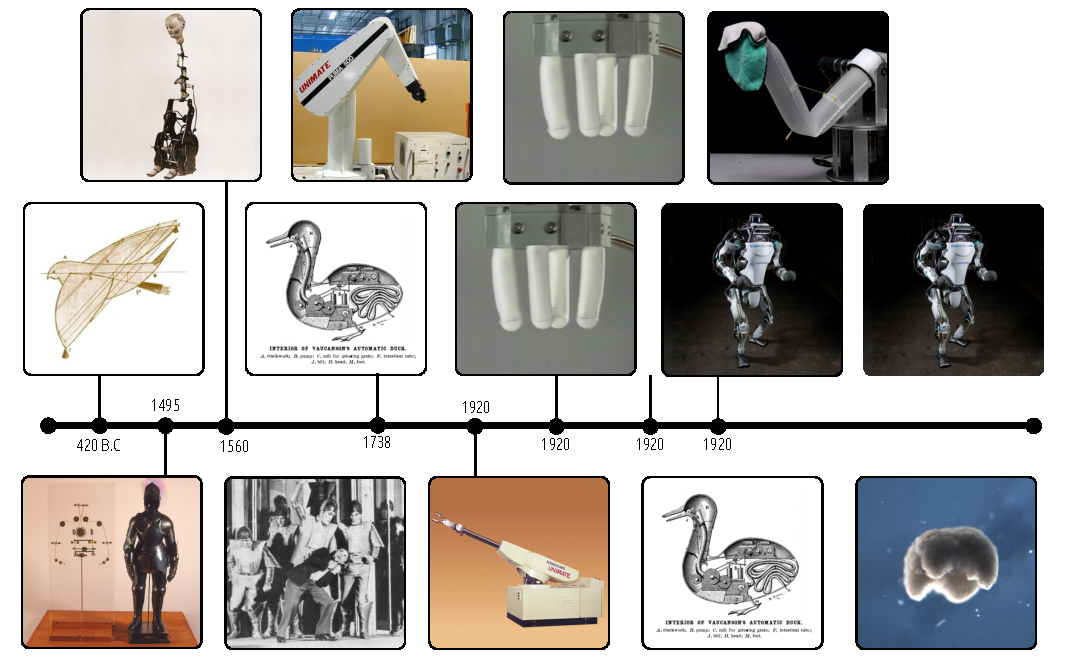
\includegraphics[width=1.11\textwidth]{./3_chapters/0_introduction/img/timeline.pdf}
\caption{A brief timeline of the state-of-the-art of robotics throughout human history. \textit{a)} One of the earliest examples of bio-mimicry -- the flying mechanical bird using steam-powered propulsion. \textit{b)} The Mechanical Knight by Leonardo Da Vinci. \textit{c)} Digesting duck patent of Jacques de Vaucanson. \textit{d)} The science-fiction play by Karel \v{C}apek on robots, who introduced the word \emph{robot} into the Oxford English Dictionary originally from his brother Josef \v{C}apek. \textit{f)} The first soft robot called Orm designed by V. Scheinman and L. Leifer. \textit{g)} The first redundant snake-like robot called Scripps tensor arm patented by V.C Anderson. }
\end{figure}
\clearpage
}

One of the earliest examples of bio-mimicry is a mechanical wooden dove developed by mathematician Archytas of Tarentum in 350 BC. According to historians, the system was driven by compressed air or an internal steam-driven engine to achieve forward propulsion, capable of traveling distances of \textapprox200 \si{\meter} (see note\footnote{It was unclear if the devices was attached to a rope, or autonomous flight was achieved.}). Archytas's invention could be considered as one of the earliest robotic systems -- a machine or device that operates automatically or by remote control -- whose main principles are somewhat analogous to nowadays \emph{drone} technology.  A millennium later, in the period of the High Renaissance, Leonardo da Vinci designed and constructed a mechanical knight around the 1490's. Such mechanical constructions were perhaps closer to conventional rigid robotics given our current robotics perspective. It is well-known that his work was built upon extensive anatomical research, which may have facilitated a deep understanding of the human body into the mechanical knight's robotic design.

\par In the 1920's, shortly after the second industrial revolution (1870 - 1914) and the first world war (1914), the first usage of the work \emph{robot} appeared -- originally meaning 'forced labor by serfs' (\ie, peasants) derived from the Czech word \emph{robota}. An common misconception is that robot implies slave, nonetheless, its origin is somewhat related. The word was popularized by Karel \v{C}apek in his play R.U.R. (Rossum’s Universal Robots) that involves an inventor named Rossum who discovers the secret of creating human-like machines. In his play, Rossom's robots assisted or fully alleviated mankind from any labor. Through human's ambition to assimilate man and machine, the robots ultimately gained the capacity for emotions. Shortly after, the robots, who were created to serve humans, have come to dominate mankind completely. The word \emph{robotics} was later solidified by Isaac Asimov, adapting the term from \v{C}apek. These works of science fiction are perhaps the fundamental groundwork of modern robotics which have led to the base practices of robotics and its corresponding academic field.

Only three decades later, in the 1950's, the first robotic arm called the 'Unimate' was employed in industry. The robot was used for manipulating metal die-casts and welding these to welding these to the main body of automobiles. Interestingly, the robot explored both electric as hydraulic-mechanical actuation, similar to nowadays popular Atlas robot (2013) by the company Boston Dynamics. Note that these robots were still controlled remotely, and rudimentary levels of closed-loop control were applied then. The 1950's also brought forth the McKibben actuators developed by Joseph Laws McKibben -- a well-known work in the field of soft robotics. These McKibben actuator consists of an inflatable inner bladder enveloped with a double-helical weave. When pressurized, the fluidic actuator converted radial expansion into uni-axial contraction since weave inhibited extensive \emph{ballooning} -- a term for undesired radial expansion. The McKibben actuators are perhaps seen as one of the first fundamental technologies that enabled soft robotics and to this day it remains a framework for many soft artificial muscle. Nevertheless, besides fluidics, there exist many other technologies employed in soft robotic motion that predate the invention of the McKibben actuator: such as thermal or chemical expansion/contraction, re-alignment of crystals, di-electric elastomers, magnetism, and naturally electro-mechanical actuation. For instance, the earliest system resambling Dielectric Elastomer Actuators (DEA) were developed W. C. R\"{o}ntgen in 1880. Although these mechanisms do not fall under the class soft robot, they are; however, categorized as soft actuators. We like to emphasize here the difference between soft actuators and soft robots in view of a terminology corresponding with the thesis:
%
\terminology{Soft actuators}{ are controllable flexible components of the constitutive soft robotic system that through external stimuli allow for motion or adaptability of compliance and/or texture.}
%
\noindent The terminology above attempts to address a common ambiguity in the field of soft robotics, that being interchangeably usage the term soft actuator and soft robot.

In 1965, the work of V. Scheinman and L. Leifer proposed a novel pneumatic robot arm named Orm -- the Norwegian word for snake. To the author's knowledge, this pneumatic robot is one of the first soft robots -- and suprisingly the system predates the first rigid redundant snake-like robots (1968). Similar to the anatomy of the snakes, the system featured 28 rubber pneumatic artificial muscle (\ie, bellows) distrubuted along the backbone (\ie, skeletal support) of the robot. The network of artificial muscles were sandwiched between steel plates to prevent disalignment. The soft robotic system could undergo three-dimensional movement by inflation or deflation of embedded pneumatic network, leading to a rich set of movements unseen in earlier robotics. The soft robot can achieve bending in any preferred direction by differential pressurization of each channel, and elongation through synchronized actuation. However, according to \cite{}, the positional accuracy of the system was poor, yet the concept of pneumatically-driven soft arms has continued. Two years later, In 1968, V.C. Anderson developed and patented one of the earliest hyper-redundant robotic manipulators.

\clearpage
\section{State-of-the-art in Soft Robotics}

\section{Problem statement}

\section{Research challenges and contribution}
\noindent \textbf{Design (Optimization)}.
\contribution{blaa}

\contribution{Validation of the proposed computational design algorithms Additive Manufacturing (AM) technologies.}

\noindent \textbf{Hyper-redundant Modeling}.
\contribution{blaa}

\noindent \textbf{Control and state estimation}.
\contribution{Development of energy-based control strategies applicable to continuum soft robotic manipulators as to allow for set-point stabilization, tracking, and grasping tasks.}

\noindent \textbf{Experimental applicability}.
\contribution{blaa}

\section{Outline of the thesis}

% \begin{figure}[t]
% \centering
% 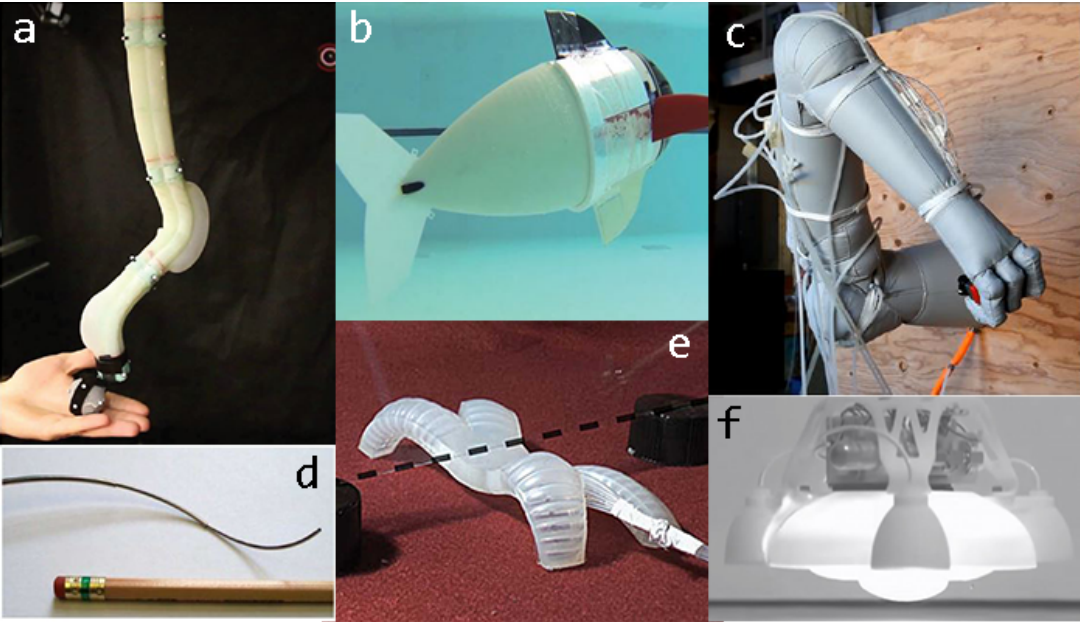
\includegraphics[width=0.98\textwidth]{./3_chapters/0_introduction/img/modern_softrobots.png}
% \caption{\textit{a)} Elepant-inspired trunk [14]. \textit{b)}, Fish-inspired aquatic robot [19]. \textit{c)}, Soft-infalatable human robot arm [13]. \textit{d)}, Concentric-tube hard continuum robot[21]. \textit{e)}, Soft quadruped robot [20]. \textit{f)}. Explosion- driven semi-soft 3D printed robot [22]. }
% \end{figure}

% Perhaps a subtle point in the terminology above, is its mention to biology.
% Although the area of soft robotics has grown exponentially since the early 2010's, the field of soft robotics dates back to the early 60's.

% \begin{figure}
% \centering
% \setlength\figurewidth{0.53\textwidth}
% \setlength\figureheight{0.25\textwidth}
% \input{./3_chapters/0_introduction/img/myfigure.tikz}
% \end{figure}

%\subsection{REF}

The first robotic manipulator arm used in the orbital environment was the Space Shuttle remote manipulator system. It was successfully demonstrated in the STS-2 mission in 1981 and is still operational today.

First soft robot: Victor Scheinman and Larry Leifer developed an air-powered robot arm called Orm, which is the Norwegian word for snake.

\begin{itemize}
  \item . F. Shulte, "The Characteristics of the Mckibben Artificial Muscle", The Application of External Power in Prosthetics and Orthetics, pp. 94-115, 1960.
  \item A. Chen, R. Yin, L. Cao, C. Yuan, H. K. Ding and W. J. Zhang, "Soft robotics: Definition and research issues," 2017 24th International Conference on Mechatronics and Machine Vision in Practice (M2VIP), 2017, pp. 366-370, doi: 10.1109/M2VIP.2017.8267170.
  \item  W. C. R\"{o}ntgen, “Ueber die durch Electricität bewirkten Form—und Volumenänderungen von dielectrischen Körpern,” Ann Phys Chem, no. 11, pp. 771-786, 1880.
\end{itemize}


%%%% Design
\cleardoublepage
\part{Design Optimization}\label{part: design}

\cleardoublepage
\part{Modeling of Soft Robots}\label{part: model}
%%!TEX root = ../../thesis.tex
%%%% CHAPTER 1 *****************************************************************
\chapter[Dynamic modeling of Soft Robots -- PCC case]{Dynamic modeling -- The Piece-wise Constant Approach}
\label{chap: chapter 1}

\blankfootnote{This chapter is based on:\\ .\disclaimer}

%%%% ABSTRACT ******************************************************************
%!TEX root = ../../thesis.tex
\chapterabstract{The motion complexity and use of exotic materials in soft robotics call for accurate and computationally efficient models intended for control. To reduce the gap between material and control-oriented research, we build upon the existing Piecewise-Constant Curvature framework by incorporating hyper-elastic and visco-elastic material behavior. In this work, the continuum dynamics of the soft robot are derived through the differential geometry of spatial curves, which are then related to Finite-Element data to capture the intrinsic geometric and material nonlinearities. To enable fast simulations, a reduced-order integration scheme is introduced to compute the dynamic Lagrangian matrices efficiently, which in turn allows for real-time (multi-link) models with sufficient numerical precision. By exploring the passivity and using the parametrization of the hyper-elastic model, we propose a passivity-based adaptive controller that enhances robustness towards material uncertainty and unmodeled dynamics -- slowly improving their estimates online. As a study case, a fully 3D-printed soft robot manipulator is developed, which shows good correspondence with the dynamic model under various conditions, e.g., natural oscillations, forced inputs, and under tip-loads. The solidity of the approach is demonstrated through extensive simulations, numerical benchmarks, and experimental validations.}


%%%% MAIN **********************************************************************
\section{Introduction} \label{sec: chap1 1_introduction}
%!TEX root = ../../thesis.tex
The field of soft robotics has attracted the interest of many researchers from different backgrounds. Soft robots use compliant and hyper-elastic materials, while the use of rigid materials is minimized. The introduction of soft materials into robotics greatly expanded the field of application for robotics. For example, due to their dexterity and environmental robustness, soft robots are often used in medical applications \cite{Polygerinos2015b, Yap2015, Asbeck2015}, adaptive grasping \cite{Galloway2016, Hughes2016}, and locomotion in uncertain environments \cite{Drotman2017}. Unlike its rigid counterpart, soft robots undergo large continuum-bodied motion that, to some extent, resembles morphologies found in nature. These morphologies arise by virtue of the low compliance in soft materials and, more importantly, the structural layout of the soft robot. As of today, many of the fundamental engineering principles in rigid robotics, like design, actuation, sensing, and control, are often not applicable to soft robotics systems. Since its inception, most of these engineering problems have remained challenging or unresolved.

Although the diversity in soft robotics is significant, ranging from adaptive grippers to soft manipulators, most topologies in soft robotics can be associated with nature or engineered geometries for minimal compliance (e.g., bellow shapes). Soft robots often mimic living creatures and their morphologies, e.g., the tentacle of an octopus \cite{Galloway2016, Wehner2016}, or the trunk of an elephant \cite{Drotman2017}. Hypothetically, the abundance of bio-mimicry in soft robotics might be associated with the design complexity of developing robots from soft materials. The large number of degrees-of-freedom and exotic mechanical nature of soft robots makes design significantly challenging, and consequently, the design process can be iterative and time-consuming \cite{Wehner2016}. Therefore, it becomes potentially advantageous to use computational tools that assist or develop appropriate soft robotic topologies given a set of user-defined requirements, like desired motion or force.

In the past, researchers have made efforts to finding morphologies through mathematics, in particular through evolutionary algorithms. The concept of automated creature designs was first introduced by Sims \cite{Sims1994}, who showed that, given a set of basic geometries, locomotive organisms could be generated from evolutionary algorithms. These virtual organisms resembled biological morphologies to some extent; however, the complexity of the material layout was limited. More recent work involving the synthesis of virtual soft robots includes Cheney et al. \cite{Cheney2013}, who successfully produced intricate locomotive morphologies using artificial neural networks and multi-material parameter spaces of active and passive soft voxels. Other work involving morphological synthesis includes \cite{Bern2019, Morzadec2019,Diepen2019}. Unfortunately, the synthesis of morphologies from previous approaches, though novel, remains only in ideal simulated environments. An accurate representation of the nonlinear material properties in soft robotics can be challenging, and in favor of computational efficiency, little detail is spent on the nonlinear nature governing soft materials. Besides, these evolutionary frameworks typically involve a network of `activation' cells or voxels that perform ideal volumetric deformation, biologically resembling muscle functionality while unfortunately lacking resemblance to conventional actuation in soft robotics, e.g., pneumatics, dielectrics, and smart metal alloys (SMA).

Reviewing previous methods, a more efficient approach for solving the optimal morphology might be founded in topology optimization. Topology optimization is the general formulation of a material distribution problem for mechanical solids, where density-based topologies arise throughout an iterative (non-convex) optimization procedure. The synthesis of compliant mechanisms through topology optimization is investigated thoroughly \cite{Sigmund2015, Gain2013, Luo2015}; however, its application to soft robotics is relatively unexplored \cite{Zhang2018,Zolfagharian2019}. Yet, to obtain meaningful topologies for soft robotics, two problems need to be addressed. Since soft robots undergo large deformations, it becomes necessary to describe the nonlinear geometrical deformations accurately. Inherent to significant deformation of soft materials is the importance of nonlinear material behavior, like hyperelasticity. Another concern is the design-dependency of the external forces, in our case, the pneumatic loads. This class of structural problems is more challenging than traditional problems since the load is continuously interacting with the adaptive interface during the iterative optimization process \cite{Wang2016, Vasista2013}. It should be mentioned that the use of compressed air or pressurized fluid is a popular actuation approach in soft robotics.

In this work, we present a novel framework for generating topologies of soft robotics. Contrary to biometry or convectional designs, finding the (optimal) material layout of the soft robot is accomplished through a gradient-based nonlinear topology optimization, where the distribution of soft materials is optimized given a user-defined objective. Our main contributions include the description of nonlinear geometrical deformation and pneumatic loading. We exploit the connectivity properties in polygonal meshes such that synchronized volumetric contraction or expansion of a group of polygonal elements can artificially mimic the geometrical loads in pneumatic actuation. The advantages of our framework in comparison to other literature are: ($i$) a better representation of pneumatic actuation in soft robotics; ($ii$) improved design convergence in contrast to evolution-based optimization methods. To our knowledge, our approach of pressure-driven nonlinear topology optimization is new for soft robotics, and its application could easily extend to other soft robotic systems. %The computational framework detailed in this work is made publicly available at \cite{Caasenbrood2019}.

The remainder of the paper is structured as follows. In section \ref{chap:fem}, we will discuss the continuum mechanics for hyper-elastic materials, followed by a description of the optimization scheme for soft robotics. In section \ref{chap:results}, we propose a numerical example for developing a soft robotic structure to illustrate the effectiveness of our approach.


\newpage
\section{Continuum dynamic model}  \label{sec: chap2 section header}
%!TEX root = ../../thesis.tex
As mentioned previously, soft robots are composed of soft bodies that may be regarded as a continuum body with (theoretically) infinitely many degrees-of-freedom (DOF). In this section, we aim to derive a compact and computationally efficient model that envelops the continuous dynamics of a soft robot through a small set of generalized coordinates $\q\in\Q$ and their respective generalized velocities \highlight{$\dq(t)\in T_{\q}\Q$} with $n$ the number of active joint variables. We base {the modeling framework on the work of Mochiyama et al.\cite{Mochiyama2003} who outlined a theoretical foundation for continuum manipulators. Their work is extended upon by including extensibility, serial-chaining of multiple soft-links, pneumatic actuation, and the introduction of nonlinear and time-dependent material behavior. Earlier modeling strategies addressing similar issues can be found in from Godage et al. \cite{Godage2015,Godage2016}, Della Santina et al. \cite{Santina2020,Santina2020b,Santina2020Pcc}, Renda et al. \cite{Renda2018}, and Boyer et al. \cite{Boyer2021}. Leveraging from the aforementioned works, the continuous dynamics of a soft robot manipulator can be written in the familiar Lagrangian form:
%
\begin{equation}
\MB(\q) \ddq + \vec{h}(\q,\dq) = \Qnc,
\end{equation}
%
where $\MB(\q)  \in \R^\nn$ denotes the generalized inertia matrix, $\vec{h}(\q,\dq) \in \R^n$ a vector of nonlinear state-dependent force contributions. In this work, a similar modeling framework is adopted; however, we propose an extension to incorporate FEM-driven data to more accurately reflect the underlying continuum mechanics -- in particular hyper-elasticity; and we propose a numerical scheme that allows for fast computation of the continuous dynamics. For completeness, we will recapitulate on the modeling approach here.

\subsection{Kinematics of elastic continuum bodies}
\noindent To represent the hyper-flexible configuration of the soft robot, let us consider a smooth spatial curve that passes through the geometric center of the continuously deformable body, as shown in Figure \ref{fig:configuration}. {In literature, this curve is called} the '\textit{backbone curve}' as it simplifies the three-dimensional deformation imposed by distributed forces acting on the elastic body. The arc-length of the backbone corresponds to the extensible length of the soft robot denoted by the variable $l(t) \in [l_{-},l_{+}]$ which we assume bounded $l_{+} \ge l \ge l_{-}$, and let $L$ be a constant denoting the {total unstressed} length of the soft robot. Next, let us introduce a spatial variable
$\sigma \in \Xs$ that belongs to the one-dimensional material domain of the backbone curve, i.e., $\Xs = [0,\, L]$. {Let it be clear that the spatial variable $\sigma$ represents the arc-length of a material coordinate along the undeformed material domain of the soft robot manipulator.}

\commentary{}{Figure here of smooth curve for p and Phi}

Given each material coordinate, we wish to find a suitable low-dimensional joint representation $q(t)$ such that the position vector $^0p$ anywhere on the continuous backbone can be written as a mapping from generalized coordinates and space into $\mathbb{R}^3$:
%
\begin{equation}
^0\pB: \Xs \times \Q(t) \to \R^3;
\end{equation}
%
and similarly the rotation matrix $^0\mat{\Phi}(\sigma,\vec{q})$ by a mapping from the generalized coordinates and space into $\SO{3}$:
%
\begin{equation}
^0\PhiB: \Xs \times \Q(t) \to \SO{3}, \label{eq:phi_map}
\end{equation}
%
where {$\SO{3}$ denotes the special orthogonal group for rotations about the origin of $\R^3$}, and $n = \dim(\vec{q})$ the state dimension. Under this notion, the position vectors $^0p(q,0)$ and {$^0\pB(L,\q)$} relate to the base and the end-effector of the soft robot, respectively. {Please note that left-sided superscript are used to indicate the frame of reference.} The set of all points on the backbone $\mathcal{P} = \left\{^0\pB \in \R^3\, |\, \sigma \in \Xs \right\}$ draws a possible {spatial} configuration of the soft robot given {a time instance $t \in \mathbb{T}$ on a finite horizon $\mathbb{T} = [0,T]$}.
%
\begin{intermez}
Despite the inherent flexibility in soft robotics, it is sometimes sufficient to express the kinematics according to the Piecewise Constant Curvature (PCC) condition. Mathematically, it implies that the curvature of the continuous body satisfies $\kappa(q,\sigma_1) = \kappa(q,\sigma_2)$ for a neighboring region of points $\sigma_1,\sigma_2 \subseteq \Xs$. As a result, this condition allows us to describe the full forward kinematics with a significantly reduced set of generalized coordinates, mitigating kinematic complexity in the model. Numerous works employ PCC models \cite{Falkenhahn2015,Katzschmann2019,Tatlicioglu2007,Marchese2016,Godage2016,Santina2020Pcc}, and depending on the degrees of elasticity, the PCC condition has been proven to be consistent for various soft robotic systems.
\end{intermez}
%
{Following this Piecewise Constant Curvature (PCC) description, let us assign a coordinate frame that twists minimally along the backbone -- a Bishop frame \cite{Bishop1975}-- parametrized by the following generalized coordinate vector:}
%
\begin{equation}
\vec{q} = \begin{pmatrix}
\,\varepsilon & \kappa_x & \kappa_y\,
\end{pmatrix}^\top \in \mathcal{Q},
\label{eq:coordinate}
\end{equation}
%
\noindent where {$\varepsilon \in \R$ is the elongation strain}, and $\kappa_x,\,\kappa_y\in\mathbb{R}$ are the curvatures or angular strains in $x$-$z$ and $y$-$z$ plane, respectively; and $\mathcal{Q} \subset \R^3$ is an admissible space on which $q$ evolves.It is worth mentioning that the joint description above is somewhat related to Renda. et al. \cite{Renda2018} who proposed a Piece-wise Constant Strain (PCS) parametrization with the exception of including the twist along the tangent.

By exploring the differential geometry of the smooth backbone curve similar to Mochiyama et al.\cite{Mochiyama2003}, we can express the spatial change of the position vector $^0 \vec{p}(0,\vec{q})$ and the orientation matrix $^0\mat{\Phi}(q,\sigma)$ for each material point $\sigma$ along the smooth backbone by
%
\begin{align}
\renewcommand*{\arraystretch}{2}{}
\frac{\partial \,^0\!\mat{\Phi}}{\partial \sigma}(\sigma,\vec{q}) & = \, ^0\mat{\Phi}(\sigma,\vec{q})\,\left[\mat{\Gamma} (\sigma,\vec{q}) \right]_{\times}, \label{eq:change_phi} \\
\frac{\partial \,^0\! \vec{p}}{\partial \sigma}(\sigma,\vec{q}) & = \, ^0\mat{\Phi}(\vec{q},\sigma) \, \vec{U}(\sigma,\vec{q}), \label{eq:change_p}
\end{align}
%
where $[\vec{\Gamma}]_\times \in \So{3}$ is a skew-symmetric matrix composed of the entries of the vector $\vec{\Gamma} \in \R^3$, and $\vec{U}\in \R^3$ a vector representing the tangent along the extensible backbone. The vectors $\vec{\Gamma}$ and $\vec{U}$ are vectors that define the differential geometry of the backbone, which are unique entries that lives in the tangent space of the rigid-body transformation group $\SE{3}$. Given the Bishop parametrization as described by \eqref{eq:coordinate}, these geometric entities yield
%
\begin{equation}
\vec{\Gamma} = \begin{pmatrix} -\kappa_y \\ \kappa_x \\ 0  \end{pmatrix}; \quad \quad \quad \vec{U} = \begin{pmatrix} \,\, 0 \,\, \\ \,\, 0 \,\, \\ \, \,\varepsilon \,\, \end{pmatrix} + \vec{U}_0,
\end{equation}
%
with $\vec{U}_0 = (0,0,1)^\top$ the unit-tangent. Now, given an initial configuration of backbone's base, i.e., $^0 \mat{\Phi}(0,\vec{q}) = \vec{\Phi}_0$ and $^0 \vec{p}(0,\vec{q}) = 0_3$, we can now solve for the position and orientation for each material coordinate $\sigma$ along the backbone:
%
\begin{align}
^0\mat{\Phi}(\sigma,\vec{q}) & = \vec{\Phi}_0\exp(\sigma [\vec{\Gamma}(\vec{q})]_\times), \label{eq:phi_exact} \\
^0\vec{p}(\sigma,\vec{q}) & = \int_0^\sigma\,^0\mat{\Phi}(\eta,\vec{q})\, \vec{U}(\vec{q}) \; d\eta, \label{eq:pos_vector}
\end{align}
%
where $\exp: \So{3} \to \SO{3}$ is the exponential map. Let it be clear that the closed-form solutions \eqref{eq:phi_exact} and \eqref{eq:pos_vector} form the forward configuration kinematics of the backbone curve. To express the forward velocity kinematic, let  $\vec{V}(\sigma,\vec{q},\dot{\vec{q}}) = \left(^\sigma \vec{\omega}^\top,^\sigma \vec{v}^\top \right)^\top \in \R^6 \cong \Se{3}
$ be the aggregate of the angular velocity and linear velocity components relative to an inertial frame at $\sigma$ (the frame of reference is denoted by a left superscript), where the space $\Se{3}$ denotes the Lie algebra of $\SE{3}$. The velocity twist is computed by the following integration procedure:
%
\begin{equation}
 \vec{V}(\sigma,\vec{q},\dot{\vec{q}}) = \Ad_{\mat{g}(\sigma,\cdot)}\inv \int_0^\sigma \Ad_{\mat{g}(\eta,\cdot)}\, J^*\! \dot{q}\;d\eta
 \,=:\, J(q,\sigma) \dot{q}, \label{eq:vel_cont}
\end{equation}
%
where $\Ad_g: \SE{3} \to \mathbb{R}^{6\times 6}$ denotes the adjoint transformation matrix regarding the rigid body transformation $g \in \SE{3}$ that maps local velocities (i.e., twist) to a frame located at $\sigma$, and $J^*$ a constant joint-axis matrix. The joint-axis matrix for an extensible and bendable PCC segment parametrized by the Bishop parameters is given by
%
\begin{equation}
\renewcommand*{\arraystretch}{1}{}
J^* := \left(\dfrac{\p \Gamma}{\p q}^\top \; \dfrac{\p U}{\p q}^\top \right)^\top  = \begin{pmatrix}
\,0 & 0 & 0 & 0 & 0 & 1 \, \\
\,0 & 1 & 0 & 0 & 0 & 0 \,  \\
\,-1 & 0 & 0 & 0 & 0 & 0 \,  \\
\end{pmatrix}^\top. \label{eq:joint-axis-matrix}
\end{equation}
%
Although we based the forward kinematics on the work of Mochiyama et al.\cite{Mochiyama2003}, the derived expression for the velocity twist in \eqref{eq:vel_cont} is analogous to the work of Renda et al.\cite{Renda2018,Renda2020}, and Boyer et al. \cite{Boyer2010,Boyer2021}. Please also note that \eqref{eq:vel_cont} gives rise to the geometric manipulator Jacobian $J(q,\sigma)
$ that defines the mapping from joint velocities to the velocity twist for a particular material point $\sigma$ on the continuous body. In continuation, let us also introduce the acceleration twist\cite{Boyer2021,Mochiyama2003,Renda2018} -- obtained through time differentiation of \eqref{eq:vel_cont}:
%
\begin{align}
\dot{V}(q,\dot{q},\ddot{q},\sigma) & = J \ddot{q} + \Ad_{g(\cdot,\sigma)} \inv \int_0^\sigma \Ad_{g(\cdot,\eta)}
\ad_{V(\cdot,\eta)} \, J^*\! \dot{q}\;d\eta \notag \\
& := J(q,\sigma)\ddot{q} + \dot{J}(q,\dot{q},\sigma) \dot{q},
\label{eq:acceleration}
\end{align}
%
where $\ad_{V} \in \mathbb{R}^{6\times 6}$ denotes the adjoint transformation regarding the velocity twist $V \in \Se{3}$. The reader is referred to Appendix A for more detailed expressions on the adjoint transformations.
%
\subsection{Euler-Lagrange equations}
\noindent Given the forward kinematics in \eqref{eq:phi_exact}, \eqref{eq:pos_vector}, \eqref{eq:vel_cont} and \eqref{eq:acceleration}, we can shift our attention to formulating the finite-dimensional dynamics of the soft robot. Our goal here is to write the spatio-temporal dynamics of the hyper-elastic soft robot as a second-order ODE into the Lagrangian form:
%
\begin{equation}
\frac{d}{d t}\left(\frac{\partial \mathcal{L}}{\partial \dot{{q}}}\right) - \frac{\partial \mathcal{L}}{\partial {q}} = {Q}^{\nc}, \label{eq:euler_largrange}
\end{equation}
%
\noindent where $\La({q},\dot{q}) := \T(q,\dot{q}) - \mathcal{U}(q)$ is the Lagrangian function, $\T \in \Rp$ and $\mathcal{U}\in \R$ the kinetic and potential energy, respectively; and $Q^{\nc} \in \mathbb{R}^n$ a vector of generalized non-conservative forces. To apply the Lagrangian formalism to a continuum dynamical system, regard an infinitesimal slice of the continuum body for each material coordinate $\sigma$ along the backbone curve. Given this notion, we embody this infinitesimal slice with an inertia tensor $
\mathcal{M} = \text{blkdiag}(\rho I_3,\mathcal{J_\sigma})$ with $\rho = m/L$ the line-density and $J_\sigma$ a tensor for the second moment of inertia. The kinetic energy can be obtained through spatial integration of its respective kinetic energy densities\cite{Boyer2010,Mochiyama2003,Tatlicioglu2007}, i.e., $\mathfrak{T} = \frac{1}{2}V^\top \mathcal{M} V
$:
%
\begin{align}
\mathcal{T}({q},\dot{{q}}) & = \frac{1}{2}\int_\Xs {V}({q},\dot{q},\sigma)^\top\,\mathcal{M}\,{V}({q},\dot{{q}},\sigma) \; d \sigma,
 \notag \\
& =  \frac{1}{2} \dot{q}^\top \int_\Xs  J({q},\sigma)^\top\,\mathcal{M}\, J({q},\sigma) \; d \sigma \, \dot{q}, \notag \\
& = \frac{1}{2}\dot{q}^\top M(q) \dot{q}. \label{eq:kinetic_energy}
\end{align}
%
Note that expression for the kinetic energy naturally gives rise to the generalized inertia matrix $M(q)$ of the Lagrangian model. By substitution of the kinetic energy into the Euler-Lagrange equation \eqref{eq:euler_largrange}, we find $M(q)\ddot{q} + C(q,\dot{q})q$ where $C(q,\dot{q})$ denotes the Coriolis matrix. Instead of computing the Coriolis matrix through the conventional Christoffel symbols\cite{Murray1994}, we adopt a computational scheme by Garofalo et al. \cite{Garofalo2013} used for serial-chain rigid manipulators, in which we replaced the finite summation of $N$ rigid-bodies by a spatial integration over the continuum domain $\Xs$:
%
\begin{equation}
C(q,\dot{q}) = \int_\Xs J(q,\sigma)^\top \Ct_{V(q,\dot{q},\sigma)}J(q,\sigma)\; + J(q,\sigma)^\top \Mt \dot{J}(q,\dot{q},\sigma) \; d \sigma,\label{eq:coriolis}
\end{equation}
%
where $\Ct_{V} = -\Ct_{V}^\top :=  \mathcal{M} \ad_{V}  - \ad_{V} ^\top \mathcal{M}$ is a skew-symmetric matrix. The computation above is slight different from existing literature\cite{Boyer2021,Renda2020} to ensure that the matrix $\dot{M} - 2C$ is skew-symmetric; the so-called the passivity condition\cite{Murray1994} for Euler-Lagrange systems (see Appendix B for proof). The importance of this property will become apparent later in the energy-based controller design. Lastly, the potential energy is given by sum of gravitational potential energy and internal elastic potential, i.e., $\mathcal{U}({q}) = \mathcal{U}_g({q}) + \mathcal{U}_e({q})
$. Since gravitational potential energy density is \rewritten{given} by $\mathfrak{U}_g = -\rho\,^0p(q,\sigma) \gamma_g$ with $\gamma_g \in \R^3$ is a vector of body accelerations, the potential energy related to gravity is obtained by spatial integration of their respective energy densities:
%
\begin{equation}
\mathcal{U}_g({q}) = - \rho \int_\Xs \,^0p(q,\sigma)^\top \gamma_g \; d \sigma.
\label{eq:potential_energy_grav}
\end{equation}
%
\noindent To model the hyper-elastic nature, lets introduce two nonlinear stiffness functions for both stretching and bending, denoted by $k_e: \R \mapsto \Rsp$ and $k_b: \R \mapsto \Rsp$, respectively. These functions allow us to describe a collective elastic behavior imposed by the hyper-elastic materials and the continuum-bodied deformation. It shall be clear that these entities are unique to the soft robot's geometry and soft material choice, and thus finding a suitable candidate model requires further analysis. Later, we will sculpt these nonlinear stiffness functions through Finite Element Methods (FEM). For now, we assume that these analytical nonlinear stiffness functions are known, and thus the (hyper)-elastic potential energy takes the form
%
\begin{equation}
\mathcal{U}_e({q}) = \int_0^{\varepsilon} k_e(\eta) \,\eta \; d \eta + \int_0^{\beta(q)} k_b(\eta)\, \eta \; d \eta,
\label{eq:potential_energy_elas}
\end{equation}
%
where $\varepsilon$ is the elongation strain, and $\beta({q}) = \kappa L (\varepsilon + 1)$ is the bending angle with the total curvature of the soft segment $\kappa = \sqrt{{\kappa_x}^2 + {\kappa_y}^2}$ (see Figure \ref{fig:configuration}).
\subsection*{Overall dynamics}
\noindent Finally, by combining \eqref{eq:euler_largrange}, \eqref{eq:kinetic_energy}, \eqref{eq:coriolis}, \eqref{eq:potential_energy_grav}, and \eqref{eq:potential_energy_elas}, the continuum dynamics of the soft robot can be casted into the familiar closed form \cite{Santina2020Pcc,Boyer2021,Renda2018,Godage2016} similar to aforementioned model (1):
%
\begin{align}
M({q})\,\ddot{{q}} + {C}({q},\dot{{q}})\,\dot{{q}} + P({q},\dot{q}) + G({q}) & = \tau(u,\delta), \label{eq:dynamic_model}
\end{align}
%
\noindent where $P = d \mathcal{U}_e/d q + R\dot{q}$ is a vector of generalized forces imposed by the deformation of the soft materials with $R \in \R^{n\times n}$ the Rayleigh damping matrix, $G = \p \mathcal{U}_g/\p q$ a vector of generalized gravitational forces, and $u \in \R^m$ the control input with the index $m$ the number of pressure inputs. The generalized input vector is chosen of the form: $\tau(u,\delta) = H u + \delta$ with $H: \R^m \mapsto \R^n$ a mapping from the input space to the joint actuation space, and $\delta(t)$ an external disturbance (e.g., unmodelled material uncertainties).
%
\begin{rmk}
Given the context of manipulators, a possible disturbance $\delta(t)$ could be an external mass applied to the tip of the soft robot. Given the kinematic relations in \eqref{eq:vel_cont} and \eqref{eq:acceleration}, one can describe the disturbance (modeled here as a point-mass located at $L$) by a state-dependent vector:
%
\begin{equation}
\delta_m = m_\delta \floor{J(\cdot,L)}_3^\top\left({\normalfont \Ad}_{g(\cdot,L)}\inv\gamma_g + \floor{\dot{V}(\cdot,L)}_3 \right),
\label{eq:delta_payload}
\end{equation}
%
where $\floor{\cdot}_3$ extracts the last three rows of a matrix or vector, and $m_\delta > 0$ the applied mass to the end-effector. It is worth recalling that the acceleration twist can be computed through the geometric Jacobian and its time derivative, i.e., $\dot{V} = J\ddot{q} + \dot{J}\dot{q}$. Indeed, the PCC condition for a soft body can only accurately describe the true dynamics if external forces produced by mass $m_\delta$ do not excessively exceed the intrinsic elastic balancing forces $P(q)$. Alternatively, a soft body can be modeled using multiple PCC curves of smaller size, similar to standard Finite Element discretization.
\end{rmk}

The actuation mapping $H$ depends on the geometry, placement, and orientation of the (pneumatic) soft actuators. Since the pneumatic chambers are aligned parallel to the backbone curve and are equally spaced along the circumference, we propose the following ansatz:
%
\begin{equation}
H: = \begin{pmatrix} \alpha_{\varepsilon} & \hdots & \alpha_{\varepsilon} \\ -\alpha_{\kappa} \cos(\phi_1) & \hdots & -\alpha_{\kappa} \cos(\phi_m) \\ \alpha_{\kappa} \sin(\phi_1) & \hdots & \alpha_{\kappa} \sin(\phi_m) \end{pmatrix},
\label{eq:mapping_H}
\end{equation}
%
where $\alpha_{\varepsilon},\alpha_{\kappa} > 0$ are system parameters representing the effective transferal of differential pressure to joint forces, and $\phi_i = (i-1)\cdot\tfrac{2\pi}{m}$ the angular inter-distance between the $m$-number of pneumatic bellows. Please note that the parameters $\alpha_{\varepsilon}$ and $\alpha_{\kappa}$ are dependent on the bellow area and radius from the bellow to the backbone curve.
%


\newpage
\section{Extension to multi-link dynamics}  \label{sec: chap2 section header}
%!TEX root = ../../thesis.tex
\noindent We previously expressed the position and velocity kinematics as explicit functions of the generalized coordinates (i.e., Bishop parameters) and their time-derivatives. This explicit dependency stems from the PCC conditions inferring the curvature is non-varying along the spatial domain $\Xs$, i.e., $\kappa(q,\sigma) = \kappa(q)$. Although sufficient for some cases, the condition is generally restrictive, and to some extent inconvenient, since the inclusion of multiple links demands piece-wise integration of the kinematics \eqref{eq:pos_vector}, \eqref{eq:phi_exact}, \eqref{eq:vel_cont}, and \eqref{eq:acceleration}. Rather than separation of integration, we can extend this PCC description by using piece-wise continuous spatial function to distinguishes multiple soft-bodied links along the continuous body of the soft robot. The idea of parametrization through shapes functions has been explored earlier by Chirikjian et al.\cite{Chirikjian1994,Chirikjian1992}, and later by Boyer et al. \cite{Boyer2021}, Della Santina et al. \cite{Santina2020b}. A similar discontinuous shape function series was used by Berthet-Rayne et al. \cite{Berthet2021} to pursue multi-body dynamics for growing continuum robots; and proposed by Chirikjian \cite{Chirikjian1992} for hyper-redundant robots earlier.

Following the aforementioned works, let us parameterize the the geometric vectors $\Gamma$ and $U$ for a $N$-link soft robot through the product of a basis of orthonormal functions $\!\{s_i\}_{i \in \N}$ and the Bishop parametrization as follows
%
\begin{align} \Gamma(q,\sigma) & = \sum^N_{i=1} s_i(\sigma) \ceil{J^*}_3
\,\tilde{q}_i, \label{eq:theta_extent} \\ U(q,\sigma) & = \sum^N_{i=1} s_i(\sigma)
\floor{J^*}_3\,\tilde{q}_i + U_0, \label{eq:h_extent} \end{align}
%
where $J^*$ is the joint-axis matrix as in \eqref{eq:adjoint_matrix}, the mathematical operators $\ceil{\cdot}_3$ and $\floor{\cdot}_3$  extract the first or last three rows of a matrix, respectively;  $\tilde{q}_i$ the joint variables of the $i$-th link, and $s_i: \Xs \mapsto \{0,1\}$ is a piece-wise continuous shape function, whose purpose is to be non-zero for a given interval on $\Xs$.
The new generalized coordinate vector becomes the aggregate of all joint variables of the multi-body soft robotic system $q =  \left(\tilde{q}_1^\top,\,\tilde{q}_2^\top,...,\,\tilde{q}_N^\top \right)^\top$ with the vector $\tilde{q}_i = (\varepsilon_{i},\, \kappa_{x,i},\,\kappa_{y,i})^\top$ relating to the Bishop parametrization of the $i$th-link. Given \eqref{eq:theta_extent} and \eqref{eq:h_extent}, we may now rewrite the velocity-twist as
%
\begin{equation} V(q,\dot{q},\sigma) = \Ad_g^{-1}
\int_0^\sigma \Ad_g J^* S(\sigma) \; d\sigma \dot{q} := J(q,\sigma) \dot{q}
\label{eq:vel_vec_dis} \end{equation}
%
where $S = (s_1,\,s_2,\,...,s_N) \otimes I_n$ is an unitary selection matrix derived from the basis of piece-wise continuous shape functions $\!\{s_i\}_{i=1}^N$. To be less ambiguous about this selection matrix $S$, lets consider a spatial coordinate $\sigma_2 \in [L_1,L_1+L_2]$ that lies on the spatial interval of the second link. Consequently, the operation $S(\sigma_2) {q} = {\tilde{q}}_2$ returns the corresponding joint variable of the second link. This selection of
generalized coordinates follows analogously for other links along the serial-chain of the soft manipulator. We provided a small library of piece-wise continuous shape functions upto $1 \le N \le 8$ links under \texttt{./src/pwf} on the open repository\cite{Caasenbrood2021}.
Now, substitution of the discontinuous variation of the geometric Jacobian in \eqref{eq:vel_vec_dis} into \eqref{eq:kinetic_energy} leads to the dynamic model of a $N$-link soft robot manipulator in the
Lagrangian form similar to \eqref{eq:dynamic_model}.


\section{Efficient solver of the soft robotic dynamics through Matrix-Differential Equations}  \label{sec: chap2 section header}
%!TEX root = ../../thesis.tex
Due to the partial differential nature of soft robots, obtaining a closed-form expression for the projected Lagrangian model in \eqref{eq:dynamic_model} can become notoriously long and complex (especially for multi-link systems). The origin of this problem stems from the integrands of inertia matrix $M(q)$ in \eqref{eq:kinetic_energy} and Coriolis forces $C(q,\dot{q})$ in \eqref{eq:coriolis}; which become highly nonlinear and therefore difficult to calculate a-priori. As a result, solving the forward dynamics using traditional solvers often deteriorates the real-time performance, and in turn its usability for closed-loop control. Inspired by Boyer et al. \cite{Boyer2021} and Godage et al \cite{Godage2016}, instead of finding an exact solution to the dynamic entries $M(q)$, $C(q,\dot{q})$ and $G(q)$, let us introduce a similar reduced-order integration scheme that produces an approximate of the dynamic model \eqref{eq:dynamic_model}. Yet, instead of using an inverse Newton-Euler algorithm (i.e., Featherstone or Hollerbach scheme) in which the Lagrangian entries are built column-wise, we propose an explicit integration scheme that efficiently computes all Lagrangian entities in parallel through a so-called Matrix-Differential Equation (MDE).

The idea here is to replace all necessary spatial integrations for the computation of the Lagrangian entities by an equivalent Matrix-Differential Equation of the form:
%
\begin{equation}
\frac{\p Z}{\p \sigma} = F(Z,\sigma), \label{eq:MDE}
\end{equation}
%
where $Z(\cdot,\sigma)$ is a matrix-valued function composed of the necessary elements for the forward kinematics and forward dynamics, and $F(Z,\sigma)$ a matrix-valued flow function that describes the spatial evolution of $Z$. Then, by choosing the appropriate initial condition for $Z(\cdot,0) = Z_0$ and numerically solving \eqref{eq:MDE} over a finite horizon $\Xs$, we can retrieve an approximate of the Lagrangian model in \eqref{eq:dynamic_model} by extracting the necessary elements from the solution $Z(\cdot,L)$.

Before describing the MDE, let us first introduce two intermediate matrices related to the computation of the manipulator Jacobian and its time-derivative, namely:
%
\begin{align}
\frac{\p B_1}{\p \sigma} & = \Ad_{g(\cdot,\sigma)}\, J^* S(\sigma), \\
\frac{\p B_2}{\p \sigma} & = \Ad_{g(\cdot,\sigma)}\ad_{V(\cdot,\sigma)}\, J^* S(\sigma)
\end{align}
%
such that they satisfy $J\dot{q} = \Ad_g\inv B_1 \dot{q}$ and $ \dot{J} \dot{q} = \Ad_g\inv B_2 \dot{q}$. Given the expressions above, we can now include a partial computation Jacobians into the MDE. By collecting all the differential relation for the forward kinematics (5), (6) and forward dynamics (14), (15), and (16), we can assign a flow function $F:= \text{blkdiag}\left(F_1,F_2 \right)$ composed of two matrices:
%
\begin{align}
F_1 & = \begin{pmatrix}
\begin{matrix}
^0 \Phi [\Gamma]_\times & ^0 \Phi U \\ 0_{3\times3} & 0_3
\end{matrix} \, \vrule & \Ad_g J^*S &\vrule\;\; \Ad_g \ad_{V} J^* S
 \end{pmatrix}, \\
F_2 & = \begin{pmatrix}
\frac{\p M}{\p \sigma} & \frac{\p C}{\p \sigma} & \frac{\p G}{\p \sigma}  \end{pmatrix},
\end{align}
%s
in which the differential form of the dynamic entities $M(q)$, $C(q,\dot{q})$, and $G(q)$ of the Lagrangian model are given by
%
\begin{align}
\frac{\p M}{\p \sigma} & = (\Ad_{g}\inv B_1)^\top \mathcal{M} (\Ad_{g}\inv B_1), \\[0.4em]
\frac{\p C}{\p \sigma} & = (\Ad_{g}\inv B_1)^\top \left[\mathcal{C}_V (\Ad_{g}\inv B_1) + \mathcal{M} (\Ad_{g}\inv B_2) \right], \\[0.4em]
\tfrac{\p G}{\p \sigma} & = (\floor{B_{1}}_3)^\top \rho \gamma_g,
\end{align}
%
We wish to stress that $F_1$ collects all elements related to the forward kinematics, whereas $F_2$ contains the dynamic entities related to the Lagrangian model. Following the spatial Matrix-Differential equation in \eqref{eq:MDE} above, its solution will be a matrix $Z := \text{blkdiag}\left( Z_1,Z_2 \right)$ composed of two smaller state matrices $Z_1$ and $Z_2$:
%
\begin{align}
Z_1 & := \begin{pmatrix}
\begin{matrix}
^0 \Phi  & ^0 p \\ 0_{3\times3} &  0_{3}
\end{matrix} \;\; \vrule & \!B_1 & \vrule & \!B_2 \;\;\;
 \end{pmatrix}, \\
Z_2 & := \begin{pmatrix} M & C & G \end{pmatrix},
\end{align}
%
Such a Matrix-Differential equation as in \eqref{eq:MDE} are not supported natively by standard ODE solvers. Therefore, an explicit second-order Runge-Kutta solver for MDEs is developed such that efficiently computes the evolution of the state matrix $Z$ along $\Xs$. The solver is written in \texttt{MATLAB} and can be found under \texttt{./src/Model.m} at Caasenbrood \cite{Caasenbrood2020}.

As for state trajectories along the temporal regime $\mathbb{T} = [0,T]$, an implicit trapezoidal integration scheme is proposed to solve the approximated continuum dynamics, which are generally less conservative on discretization to preserve numerical stability. Here implicit schemes are favored over explicit scheme, since a coarser time integration can significantly increase real-time performance. In addition, to further boost performance of the temporal integration, a cost-effective approximation of the Hessian is introduced. For more detail, see Appendix C for more detail.


%%%%%%%%%%%%%%%%%%%%%%%%%%%%%%%%%%%%%%%%%%%%%%%%%%%%%%%%%%%%%%%%%%%%%%%%%%%%%%%%


\part{Control and Sensing Strategies}\label{part: control}
% \cleardoublepage
% \part{Name of second part}\label{part: part2}
% \include{3_chapters/1_introduction/}
% %
% \cleardoublepage
% \part{Conclusions and recommendations}\label{part: closing}
% \chapter{Conclusions and recommendations}
\label{chap: conclusions}
\thispagestyle{empty}

\section{Conclusions}

\lipsum[20-23]
Restate your thesis objective.

\vspace*{3mm}
\objective{State the objective of your PhD research here.}



%**********************************************************************%


\section{Recommendations}

\lipsum[1-4]

%%%% APPENDIX ******************************************************************
\appendix
\cleardoublepage
\part{Appendices}
\definecolor{thumbcolor}{gray}{0.4}     % Change the color of the thumb index tags to gray
\chapter{Appendix name}
\label{app: appendix 1}

\section{Section header}

\lipsum[1-4]


%%%% BACK MATTER ***************************************************************
\isstarredchaptertrue           % This state variable is used for creating the thumb index by indicating that the following chapter is not numbered (i.e. \chapter*{})
\bookmarksetup{startatroot}
\addtocontents{toc}{\bigskip}%
%!TEX root = ../thesis.tex
%\footnotesize
{\fontsize{9pt}{10pt}\selectfont

\bibliographystyle{ieeetr}
%\bibliographystyle{apalike}
\cleardoublepage
\phantomsection
\addcontentsline{toc}{chapter}{\bibname}
\bibliography{5_bibliography/MyBib}
%
}

\normalsize

\chapter*{Acknowledgments}
\addcontentsline{toc}{chapter}{Acknowledgements}
\markboth{Acknowledgements}{Acknowledgements}
\vspace{-5mm}

% When I was young I always wanted to pursue a scientific career. The pursuit of achieving my doctorate's degree has been by far the largest and heaviest stepping stone in that career. I have been extremely fortune not only in the opportunities that (sometimes seemingly) I've been given but also with the relations that have fruited over the past years.

% It is no secret that without these individuals I'd be unable to reach these achievements in life.

As I embark on the end of my PhD journey, I am somewhat reminded of the Latin motto of the Eindhoven University: ``\textit{Mens agitat molem},'' which translates to ``\textit{Mind moves the mass}.'' This beautiful phrase perhaps encapsulates the essence of my academic pursuit, where other minds played a pivotal role in influencing and reshaping the world around me. Throughout my PhD, I have had the extreme privilege of connecting with various brilliant scholars, mentors, fellow students, and (new) friends who have expanded my understanding within the areas of research, but more importantly, beyond such scopes. ``textit{Mens agitat molem}'' is evident in the collaborative discussions, debates, exchanges of ideas, and connections that have fueled my personal growth and pushed me -- the metaphorical ``mass'' -- forward throughout these years.

First, I would like to express my gratitude to my first promotor. Henk, ik wil je bedanken  voor alle mogelijkheden die je mij hebt geboden tijdens en vooraf mijn promotietraject. Ik heb het gevoel dat onze visie voor het veld 'soft robotics' altijd parallel heeft gelopen, en dit heeft niet alleen geleid tot een uiterst prettige samenwerking, maar heeft mij ook de vrijheid gegeven om mijzelf als onderzoeker vrij te ontwikkelen. Je scherpe opmerkingen, maar vooral ook je humoristische inbreng, werden zeer gewaardeerd. Je begeleiding, steun, en expertise hebben mij geholpen om mijn promotietraject tot een succesvol einde te brengen. Bedankt voor alles.

Secondly, I would like to express my sincere appreciation to my co-promoter, Sasha. I am immensely grateful for your unwavering support and open-mindedness throughout the years, but above all, for your remarkable patience with me. You have consistently provided me with the freedom to explore new ideas, and we have engaged in numerous captivating discussions connected to the realm of soft robotics. Furthermore, I deeply value the time and availability you have dedicated to me, even without prior notice. This has truly made me feel that your doors are always open – a practice that I have come to embrace with my own students over the course of my Ph.D. career.

My sincere gratitude also goes to the committee members who have been part of reviewing the thesis and participating in the public defense: Jaap den Toonder, Gijs Krijnen, Bas Overvelde, and Anibal Ollero; and my gratitude to Patrick Anderson who agreed to chair the defense ceremony.

I would also like to express my gratitude to the members of the {Wearable Robotics} project. Herman, thank you for assembling such a wonderful and diverse group of researchers. The monthly telecoms and yearly consortia that brought us together were inspirational and insightful, and I thoroughly enjoyed the platform that was given for discussions and collaboration. Ali, thank you for all the fruitful collaboration, and I am proud of our collaboration and publication, which has become a chapter of your dissertation. What an honor to be part of your doctoral work! Mariska, thank you for all your interesting input and the opportunities you have given Ali and me to gain insight into the clinical world. I also want to thank the other fantastic researchers from Twente: Martijn, Cristina, Alejandro, Ander, Michelle, and the folks from Delft, Cor, and Wouter; you guys are truly inspiring engineers.

I am deeply grateful to my wonderful ex-colleagues with whom I have had the pleasure of working on various courses: Astrid, Bayu, Carlos, Ines, Nathan, Matt, and Ruben, and a few others I'd like to mention separately. Alessandro, I want to express my heartfelt appreciation for our collaboration on the robotics course. Your consistent interest in my project and the occasional interesting emails on related research topics have been truly valuable. Irene, bedankt voor onze vlekkeloze samenwerking tijdens de Haptics en voor het verwelkomen in jullie onderzoeksgroep en lab. Rob, ik heb oprecht genoten van onze samenwerking bij Dynamics, maar wat ik het meest bewonder, is jouw standvastige aanwezigheid tijdens de ``Vrijmibo'', zowel in persoon als virtueel. Gerard, bedankt voor de boeiende discussies die we hebben gehad onder het genot van een kopje koffie. Ik wil ook graag Harry, Peter (2x) erkennen voor hun lab ondersteuning. Tot slot, Geertje, hartelijk dank voor alles wat je hebt gedaan. De zorg die je hebt voor onze groep, maar ook voor elk individu, blijft niet onopgemerkt. Jij bent werkelijk de steunpilaar van onze groep. Thank you all for making my time at the TU/e memorable and rewarding.

To the students I had the pleasure of supervising: Erwin, Sef, Willem, Has, and Yoshi, and a few others I'd like to mention separately. Benn, I feel extremely lucky that, out of all the students who rejected my B.Sc project proposal, you were the one to give it a shot. Call it fate. I was thrilled to hear you had joined our group, and I now know the ``Vrijmibo'' is in good hands. Hoang, it was a pleasure supervising you. Thanks for the ergonomic mouse which I am still using while finishing up these last pages. Also, Tijn, thanks for the extremely nice collaboration. It was a pleasure reading all of your ``extensive'' reports, and I was surprised by your kind words in the acknowledgements of your thesis.

I would also like to express my heartfelt gratitude to my former office mates. Tom, ik ben dankbaar voor de begeleiding en steun die je hebt geboden tijdens de begindagen als jonge promovendus. Ook onze samenwerkingen op jouw CAD-gerelateerde projecten voor de fiets waren echt vermakelijk. Rinus, bedankt voor jouw luisterend oor en betrokkenheid bij allerlei interessante discussies op kantoor. Ik zal onze uitgebreide whiteboard discussies missen, die immers essentieel zijn geweest voor de vormgeving van deze scriptie. Jouw aanwezigheid als kantoorgenoot is waardevol geweest, vooral wanneer ik een extra `\emph{mind}' nodig had om mentale blokkades te verhelpen. Ana, I will cherish the memories of our delightful coffee breaks and the engaging discussions we had, particularly the ones we shared digitally from my kitchens during the pandemic. I am also grateful for the opportunity to publish together. Lastly, I would like to acknowledge Guo and Nishant, albeit our time together in the office was brief, your contributions and camaraderie were greatly appreciated. 

Also thanks to all my fellow Ph.D.s who've I had to pleasure to share the occasional coffee. Thanks to my other coworkers from D\&C: Alexander, Andy, Bas, Dirk, Dipankar, Fahim, Haleh, Jizheng, Joey, Kaidong, Kevin, Lars (2x), Luuk (2x), Maarten, Philipp, Rapha\"{e}l, Raul, Roeland, Rigo, Sebastiaan, Semih, Viral, Wouter (2x), and Yuzhe; and the folks from CST: Bardia, Casper, Hao, Jilles, Koen (2x), Leontine, Maurice, Max, Nard, Noud, Paul, Puck, Roy, Sven, and Tomas. Also thanks to all the older former colleagues that have improved the Ph.D. experience significantly: Alex, Chyannie, Daniel (2x), Frans, Igor, Kirill, Lennart, Leroy, Michiel, Quentin, Robert, Rishi, Ruud, Sajad, Suraj, and Veronica.

There are a few colleagues I'd like to mention separately. Krishna, your unbreakable optimism and your laugh that echoes through the halls of Gemini-South are seriously infectious and uplifting. Thanks for all that you have organized. Dario and Alessia, thanks for all the nice Italian coffee and cookies -- grazie mille! Jari, hartelijk dank dat je me feitelijk gratis hebt meegenomen naar Rammstein. Het was een mooie gelegenheid waarop mijn ``lange-haar-fase'' zijn vruchten heeft afgeworpen. Ruud, hartelijk dank voor je sporadische bezoeken aan mijn kantoor, je aansporing om die ene keer naar de sportschool te gaan en al onze interessante filosofische discussies. Ricky, het was altijd een genoegen wanneer je langs kwam op kantoor. Mischa, it was a pleasure being my partner-in-crime when infiltrating the Benelux meeting. It was a legendary evening, by far the best Benelux meeting for me! Naturally, I have to extend my gratitude to Venkata for not showing up, so I could borrow his name tag, and all the other PhDs who heroically gifted all their beers to me. Femke and Mahboubeh, thank you for the fruitful collaborations. I was thrilled to see more people starting to work on soft robotics within our group, and I am delighted that we had the opportunity to publish together. A small shoutout to the people at AMOLF: Alberto, Mannus, Paul, Sergio, and (the legendary) Shibo; for a memorable experience at last year's Dutch Soft Robotics Symposium in Twente.
The same naturally applies to the folks of the Reshape group. Also special thanks to those that celebrated my hand-in date, those that pleasantly surprised me on my 30\textsuperscript{th} birthday, and the regulars at the ``\textit{VrijMiBo}''. To all of you, my heartfelt thanks for transforming my time at the University into an unforgettable, rewarding experience full of cherished friendships.

Camiel, ook bedankt voor al die vroege ochtendtreinritten. De mogelijkheid om alles aan jou voor te leggen hebben mij veel mentale rust gegeven en hebben deelsgeleid tot het succesvol afronden van dit boekje. Falco, bedankt voor je constante interesse, suggesties voor zelfverbeteringsboeken, game- en pizzanachten. Roos, bedankt voor je steun en levensadvies. Jullie zijn geweldige vrienden geweest gedurende al die jaren, een echte vangst! Martijn en Bob, bedankt voor alle whiskey-(maar voornamelijk speciaal bier)-avonden. Dank aan Anne en Britt voor alle ``gamy-gamy'' avonden, filmavonden, tripjes Groningen, en natuurlijk onze magische reis naar Londen -- kan niet wachten op een vervolg (of trilogie). Jullie vriendschap is essentieel motivatievoer geweest voor dit boekje. Gijs en Bob, bedankt voor het accepteren van de rol van paranymph, met twee van mijn oudste vrienden aan mijn zijde heeft de tegenpartij geen kans. Mijn dankbaarheid strekt zich natuurlijk ook uit naar de andere oldies Roel, Michel, en ook Panda. Xavier, bedankt voor al je frequente herinneringen om af te spreken. Dank aan Dominique voor het organiseren van al deze geweldige reizen en avonturen die we de afgelopen plus-tien jaar hebben gehad, grotendeels dankzij jouw fantastische organisatietalent. De recente Ardennen en Londen trip waren de hoognodige pauzes waar ik zo naar verlangde tijdens mijn promotieonderzoek. Ties, bedankt dat je altijd mijn vaste aanspreekpunt bent geweest voor alles wat met concerten te maken heeft. En vanzelfsprekend gaat mijn dank ook uit naar de andere old-timers: Cynthia, Siem, Jeffrey, Etienne, Jolijn en Dennis. Diem en Lissane, bedankt voor alle gezelligheid en de geweldige Foals LP die jullie hebben geschonken - mijn favoriet tot heden.

Manu und Nina, vielen Dank f\"{u}r eure Gastfreundschaft in R\"{o}dern, die Biere und das fantastische deutsche Essen, die speziellen, thematischen Geburtstagspartys - nat\"{u}rlich war Big Lewboski meine Lieblingsparty - und die Brettspielabende. Johannes, vielen Dank f\"{u}r dein wissenschaftliches Interesse, und Sarah, danke f\"{u}r deinen herzlichen Empfang in die Familie. Regina und Karsten, danke, dass ihr mich so in eure Familie einbezogen habt, so dass ich mich dazugeh\"{o}rig gef\"{u}hlt habe.

Mam, ik wil je enorm bedanken voor al je ongelofelijke support in zowel mijn persoonlijke ontwikkeling als mijn carrière. Jouw constante aanmoediging en steun vanaf het begin hebben eindelijk hun vruchten afgeworpen. Ik ben enorm dankbaar en trots dat ik jou als mijn moeder heb. Ook wil ik graag mijn broer, Myron of Madji, bedanken. De steun die jullie hebben aangeboden is ongelofelijk waardevol en heeft geleid tot het stand komen van deze thesis. Zonder jullie zou ik dit nooit hebben kunnen bereiken. Pap, bedankt voor je interesse en steun gedurende de afgelopen jaren. Jouw betrokkenheid heeft me altijd gemotiveerd en ge\"{i}nspireerd om het beste uit mezelf te halen. Ook Rachel verdient een speciale dankjewel, je betrokkenheid in onze familie is goud waard.

Also, thanks to those few I might have forgotten to mention. I have an exceptionally bad memory for names, but I won't easily forget a face.

Last but not least, my dearest Miriam, words cannot express the joy I have felt having you by my side during these ``\textit{tough}'' albeit ``\textit{adventurous}'' times. You were the light that has guided my soul to a safe and happy haven, and without you, I was probably not able to make it.

\begin{flushright}
Brandon Caasenbrood \\
Eindhoven, September 2023
\end{flushright}  
%!TEX root = ../thesis.tex
%*********************************************************************************%
\chapter*{List of publications}
\addcontentsline{toc}{chapter}{List of publications}
\markboth{List of publications}{List of publications}
\newcommand{\ipj}{(\textit{in preparation for journal submission})}
\newcommand{\cur}{(\textit{under review})}
\newcommand{\sbm}{(\textit{submitted})}
\newcommand{\acp}{(\textit{accepted})}
\newcommand{\inp}{(\textit{in press})}

% \section*{Preliminary titles}
% \begin{enumerate}[leftmargin=2.5mm]
% \item A Control-oriented Perspective on Design and Modeling of Soft Robotic Systems;
% \item Towards a Unified Framework for Design and Model-based Control of Soft Robots;
% \item Addressing the Open Challenges in Soft Robotics: from Design to Model-based Control
% \item Design and Control Strategies for Soft Robotic Systems;
% \item Design, Modeling, Simulation and Control of Soft Robots.
% \item Design, Modeling and Control Strategies for Soft Robotics Systems;
% \item (Soft Manipulators/Soft Robotic Manipulators?)
% \end{enumerate}
%
% \section*{Preliminary committee members}
% \begin{itemize}[leftmargin=4mm]
% \item prof. J. den Toonder (TU/e, Microsystems, ICMS) \vspace{-2mm}
% \item dr. R. Luttge (TU/e, Microsystems) - Backup for Jaap \\ ............................................................................................... \vspace{-2mm}
% \item prof. G. Krijnen (Twente University) Technologies) \vspace{-2mm}
% \item prof. C.C.L. Wang (Delft University) \vspace{-2mm} \href{https://ieeexplore.ieee.org/document/9426391}{[1]}, \href{https://www.researchgate.net/publication/347965436_Jacobian-based_learning_for_inverse_kinematics_of_soft_robots}{[2]}
% \item prof R. Carloni (Rijksuniversiteit
% Groningen) - backup for Gijs \\ ............................................................................................... \vspace{-2mm}
% \item dr. E. Franco (Enrico, Imperial College London) \vspace{-2mm} \href{https://link.springer.com/article/10.1007/s11071-021-06817-1}{[1]}, \href{https://ieeexplore.ieee.org/document/9638969}{[2]}
% \item prof. H. Mochiyama (University of Tsukuba) \href{https://www.sciencedirect.com/science/article/pii/S2405896320328226?via%3Dihub}{[1]}, \href{https://ieeexplore.ieee.org/document/1242160}{[2]} \vspace{-2mm}
% \item dr. C. Duriez (INRIA Lille) \href{https://hal.inria.fr/hal-01370347/document}{[1]},\href{https://hal.archives-ouvertes.fr/hal-03192168/document}{[2]}\vspace{-2mm}
% \item prof. R. Katzschmann (ETH Zurich) \href{https://www.liebertpub.com/doi/pdfplus/10.1089/soro.2014.0022}{[1]},\href{https://arpi.unipi.it/retrieve/handle/11568/996018/683882/Final%20manuscript%20IEEE.pdf}{[2]}\vspace{-2mm}
% \item dr. S. Grazioso (University of Naples) \href{https://pubmed.ncbi.nlm.nih.gov/30481112/}{[1]} \vspace{-2mm}
% \item dr. M. Bächer (ETH Zurich) \href{https://pubmed.ncbi.nlm.nih.gov/31891526/}{[1]},\href{https://ieeexplore.ieee.org/document/9312179}{[2]}
% \item Antonio Bicchi - Italian
% \item Annibal Olero - Spain
% \item Bas Overvelde??
% \end{itemize}
\vspace{-10mm}
%*********************************************************************************%
\section*{Peer-reviewed journal articles}
\begin{itemize}[leftmargin=4mm]
  \item B. Caasenbrood, A. Pogromsky and H. Nijmeijer, “\textit{Generative Design of Soft Robotic Actuators -- a Gradient-based Approach}”, Frontiers in Robotics and AI, 2022. \ipj;
\item B. Caasenbrood, A. Pogromsky and H. Nijmeijer, “\textit{Reduced-order Cosserat Models for Soft Robotic
 Systems using FEM-driven Shape Reconstruction}”, Robotics and Automation Letters, 2022. \ipj;
%\item B. Caasenbrood, A. Amoozandeh Nobaveh, M. Janssen, A. Pogromsky, J. Herder, and H. Nijmeijer “\textit{An Energy-efficient Gravity-balancing Wrist Exoskeleton by exploring Compliant Beams and Soft Robotic Actuation},” Wearable Technologies. \ipj;
\item A. Amiri, B. Caasenbrood, D. Liu, N. van de Wouw, and I. Lopez Arteaga, "\textit{An Electric Circuit Model for the Nonlinear Dynamics of Electro-active Liquid Crystal Coatings}", Applied Physics Letters, 2022. \sbm;
\item  B. Caasenbrood, A. Pogromsky and H. Nijmeijer, “\textit{Energy-shaping Controllers for Soft Robot Manipulators through Port-Hamiltonian Cosserat Models}”, SN Computer Science Springer, 2022. \acp;
\item B. Caasenbrood, A. Pogromsky and H. Nijmeijer, "\textit{Control-oriented Models for Hyper-elastic Soft Robots through Differential Geometry of Curves}”, Soft Robotics, 2022.
\end{itemize}

%*********************************************************************************%
\section*{Peer-reviewed articles in conference proceedings}
\begin{itemize}[leftmargin=4mm]
\item B. Caasenbrood, F.E. van Beek, H. Khanh Chu, and I.A. Kuling, “\textit{A Desktop-sized Platform for Real-time Control Applications of Pneumatic Soft Robots},” IEEE International Conference on Soft Robotics, RoboSoft 2022, pp 217-223.
\item A. Amoozandeh Nobaveh, and B. Caasenbrood, "\textit{Design Feasibility of an Energy-efficient Wrist Exoskeleton
using Compliant Beams and Soft Actuators}", Proceedings of the 18th International  Consortium for Rehabilitation Robotics, 2022 (accepted).
\item B. Caasenbrood, A. Pogromsky and H. Nijmeijer, "\textit{Energy-based control for Soft Robots using Cosserat-beam models}”, Proceedings of the 18th International Conference on Informatics in Control, Automation and Robotics, 2021, pp. 311–319.
\item B. Caasenbrood, A. Pogromsky and H. Nijmeijer, "\textit{A Computational Design Framework for Pressure-driven Soft Robots through Nonlinear Topology Optimization}," 2020 3rd IEEE International Conference on Soft Robotics, 2020, pp. 633-638.
\item B. Caasenbrood, A. Pogromsky and H. Nijmeijer, “\textit{Dynamic modeling of hyper-elastic soft robots using spatial curves},” IFAC World Congress, IFAC-PapersOnLine, 2020, pp. 9238-9243.
\end{itemize}

\section*{Invited Talks and non peer-reviewed abstracts}
\begin{itemize}[leftmargin=4mm]
\item B. Caasenbrood, talk on  “\textit{3D-printed Soft Robotics},” Symposium on Robotic Technologies, Ultimaker, 2022. (invited speaker).
\item B. Caasenbrood, \texttt{SOROTOKI}: \textit{an open-source MATLAB toolkit for Design, Modelling and Control of Soft Robots},”   4TU Federation`s Symposium on Soft Robotics, Delft University, 2022. (invited speaker).
\item B. Caasenbrood, “\texttt{SOROTOKI}\textit{: an Open-source Toolkit for Soft Robotics written in MATLAB},”  IEEE International Conference on Soft Robotics, RoboSoft 2022, Edinbrugh. (poster presentation). \texttt{Best Poster Award}
\item B. Caasenbrood, C. Della Santina, and A. Pogromsky, “\textit{Workshop on Model-based Control of Soft Robots},” European Control Conference (ECC), 2021. (main organizer).
\item B. Caasenbrood, talk on  “\textit{Towards Design and Control of Soft Robotics},” 4TU Symposium on Soft Robotics (digital), 2020. (invited speaker).
\item B. Caasenbrood, talk on  “\textit{3D-printed Soft Robotics},” Symposium on Robotic Technologies, 2019. (invited speaker).
\item B. Caasenbrood, A. Pogromsky and H. Nijmeijer, talk on  “\textit{Forward Dynamics of Hyper-elastic Soft Robotics},” 39th Benelux Meeting on Systems and Control, 2019. (abstract).
\item B. Caasenbrood, A. Pogromsky and H. Nijmeijer, talk on  “\textit{Dynamical modeling and control of continuum soft robots},” 37th Benelux Meeting on Systems and Control, 2018. (abstract).
\end{itemize}

%*********************************************************************************%
\chapter*{Curriculum Vitae}
\addcontentsline{toc}{chapter}{Curriculum Vitae}
\markboth{Curriculum Vitae}{Curriculum Vitae}




\newpage {~}
\thispagestyle{empty}

\ifprint{}
\else
\newpage {~}
\thispagestyle{empty}
\fi

%%%% BACK **********************************************************************
\cover{thesis_back.pdf}    % Adds your thesis' back cover if the option 'print' is NOT used. Printing companies require the thesis cover to be supplied separately and in a different format. Definition of \cover{} is given in commands.tex.

\end{document}
%%%% THAT's ALL FOLKS **********************************************************
